\documentclass[10pt,journal,compsoc]{IEEEtran}
% \usepackage[margin=1.3in]{geometry}
% \addtolength{\topmargin}{-.2in}
% \addtolength{\topmargin}{-.2in}
\usepackage{amssymb}
\usepackage{amsmath,amsthm}
\usepackage{url}
%\usepackage{tabularx}
\usepackage[table]{xcolor}
\usepackage{color}
\usepackage{caption}
\usepackage{algorithm}
\usepackage{algorithmicx}
% \usepackage{algorithm2e}
\usepackage{graphicx}
\usepackage{pgfplots}
\usepackage{comment}
\usepackage{mathrsfs} 
\usepackage{subcaption}
\usepackage{threeparttable}
\usepackage{multirow}
\usepackage{array}
\usepackage{mathrsfs} 
\usepackage{booktabs}

\newtheorem{Theorem}{Theorem}
\newtheorem{Definition}{Definition}
\newtheorem{Observation}{Observation}


\title{Scalable Key-Aggregate Cryptosystem for Secure Online Data Sharing on the Cloud}
\begin{document}
% 
% \author{}
% \institute{}

\author{Sikhar Patranabis, Yash Shrivastava and Debdeep Mukhopadhyay
\\Department of Computer Science and Engineering\\ Indian Institute of Technology Kharagpur
\\\{sikhar.patranabis, yash.shrivastava, debdeep\}@cse.iitkgp.ernet.in}
\maketitle
% \toctitle{Lecture Notes in Computer Science}
% \tocauthor{Authors' Instructions}


\begin{abstract}

Online data sharing for increased productivity and efficiency is one of the primary requirements today for any organization. The advent of cloud computing has pushed the limits of sharing across geographical boundaries, and has enabled a multitude of users to contribute and collaborate on shared data. However, protecting online data is critical to the success of the cloud, which leads to the requirement of efficient and secure cryptographic schemes for the same. Data owners would ideally want to store their data/files online in an encrypted manner, and delegate decryption rights for some of these to users, while retaining the power to revoke access at any point of time. An efficient solution in this regard would be one that allows users to decrypt multiple classes of data using a single key of constant size that can be efficiently broadcast to multiple users. In this paper, we address this problem by proposing  a dynamic, scalable and efficient key aggregate encryption scheme with provable security and user revocation properties. We lay special focus on how the scheme can be actually deployed on the cloud for multiple data owners and data users. We present simulation results to prove the efficiency of the scheme and compare its performance with other existing cryptosystems for online data sharing in literature.

\begin{IEEEkeywords}
 Cloud Computing, Data Sharing, Data Security, Key-Aggregate Cryptosystem, Provable Security, Scalability, Revocation
\end{IEEEkeywords}

% \noindent{\textbf{Keywords:}} Key-Aggregate Cryptoystem, Online data sharing, Semantic security, Dynamic access rights
\end{abstract}

\section{Introduction}
\label{sec:Intro}

\IEEEPARstart{T}{he} recent advent of cloud computing has pushed the limits of data sharing capabilities for numerous applications that transcend geographical boundaries and involve millions of users. Governments and corporations today treat data sharing as a vital tool for enhanced productivity. Cloud computing has revolutionized education, healthcare and social networking. Perhaps the most exciting use case for cloud computing is its ability to allow multiple users across the globe share and exchange data, while saving the pangs of manual data exchanges, and avoiding the creation of redundant or out-of-date documents. Social networking sites have used the cloud to create a more connected world where people can share a variety of data including text and multimedia. Collaborative tools commonly supported by cloud platforms and are extremely popular since they lead to improved productivity and synchronization of effort. The impact of cloud computing has also pervaded the sphere of healthcare, with smpartphone applications that allow remote monitoring and even diagnosis of patients. In short, cloud computing is changing various aspects of our lives in unprecedented ways.

Despite all its advantages, the cloud is susceptible to privacy and security attacks, that are a major hindrance to its wholesome acceptance as the primary means of data sharing in today’s world. According to a survey carried out by IDC Enterprise Panel in August 2008 \cite{panelcloud}, Cloud users regarded security as the top challenge with $75\%$ of surveyed users worried about their critical business and IT systems being vulnerable to attack. While security threats from external agents are widespread, malicious service providers must also be taken into consideration. Since online data almost always resides in shared environments (for instance, multiple virtual machines running on the same physical device), ensuring security and privacy on the cloud is a non trivial task. When talking about security and privacy of data in the cloud, it is important to lay down the requirements that a data sharing service must provide in order to be considered secure. We list down here some of the most primary requirements that a user would want in a cloud-based data sharing service:

\begin{itemize}
 \item \emph{Data Confidentiality}: Unauthorized users (including the cloud service provider), should not be able to access the data at any given time. Data should remain confidential in transit, at rest and on backup media.
 
 \item \emph{User revocation}: The data owner must be able to revoke any user's access rights to data the without affecting other authorized users in the group. 
 
 \item \emph{Scalability and Efficiency}: Perhaps the biggest challenge faced by data management on the cloud is maintaining scalability and efficiency in the face of immensely large user bases and dynamically changing data usage patterns.
 
 \item \emph{Collusion between entities}: Any data sharing service in the cloud must ensure that even when certain malicious entities collude, they should still not be able to access any of the data in an unauthorized fashion. 

\end{itemize}

 
\begin{figure*}
\centering
\captionsetup{font=scriptsize}
\includegraphics[scale=0.4]{Figs/KeyAgg.png}
\caption{Example of Online Data Sharing}
\label{fig:intro}
\end{figure*}

A traditional way of ensuring data privacy is to depend on the server to enforce access control mechanisms \cite{chow2012spice}. This methodology is prone to privilege escalation attacks in shared data environments such as the cloud, where data corresponding to multiple users could reside on the same server. Current technology for secure online data sharing comes in two major flavors - trusting a third party auditor \cite{cryptoeprint:2009:579}, or using the user's own key to encrypt her data while preserving anonymity \cite{chow2012dynamic}. In either case, a user would want a reliable and efficient cryptographic scheme in place, with formal guarantees of security, high scalability and ease of use. The main challenge in designing such a cryptosystem lies in effective sharing of encrypted data. A data sharing scheme on the cloud is only successful if data owners can delegate the access rights to their data efficiently to multiple users, who can then access the data directly from the cloud servers. Figure \ref{fig:intro} describes a realistic online data sharing set-up on the cloud. Assume that the data owner is using an online data sharing service such as Microsoft OneDrive \cite{shallman2014up} to store her research documents. She wishes to add an additional layer of security for her data by storing them in an encrypted fashion. Now, she intends to share specific subsets of these documents with different collaborators. For this, she needs to provide each of her collaborators with decryption rights to specific classes of the data that they are authorized to access. She might also wish to dynamically update the delegated access rights based on changes to the data/credibility issues. The challenge therefore is to provide her with a secure and efficient online \emph{partial} data sharing scheme that allows updates to user access rights on the fly.

A n\"{a}ive (and extremely inefficient) solution is to have a different decryption key for each ciphertext class, and share them accordingly with users via secured channels. This scheme is not practically deployable for two major reasons. Firstly, the number of secret keys would grow with the number of data classes. Secondly, any user revocation event would require Alice to entirely re-encrypt the corresponding subset of data, and distribute the new set of keys to the other existing valid users. This makes the scheme inefficient and difficult to scale. Since the decryption key in public key cryptosystems is usually sent via a secure channel, smaller key sizes are desirable. Moreover, resource constrained devices such as wireless sensor nodes and smart phones cannot afford large expensive storage for the decryption keys either. Not many of the present cryptosystems seem to address this issue of reducing the decryption key size for online data sharing schemes, as we describe next.


\subsection{Related Work}
\label{subsec:relatedwork}

In this section we present a brief overview of public and private key cryptographic schemes in literature for secure online data sharing. While many of them focus on key aggregation in some form or the other, very few have the ability to provide constant size keys to decrypt an arbitrary number of encrypted entities. One of the most popular techniques for access control in online data storage is to use a pre-defined hierarchy of secret keys in the form of a tree-like structure, where access to the key corresponding to any node implicitly grants access to all the keys in the subtree rooted at that node \cite{tzeng2002time,ateniese2012provably,sandhu1988cryptographic,sun2004scalable,atallah2009dynamic,ateniese2012provably}. A major disadvantage of hierarchical encryption schemes is that granting access to only a selected set of branches within a given subtree warrants an increase in the number of granted secret keys. This in turn blows up the size of the key shared. Compact key encryption for the symmetric key setting has been used in \cite{benaloh2009patient} to solve the problem of concisely transmitting  large number of keys in the broadcast scenario. However, symmetric key sharing via a secured channel is costly and not always practically viable for many applications on the cloud. Proxy re-encryption is another technique to achieve fine-grained access control and scalable user revocation in unreliable clouds \cite{ateniese2006improved,liu2011reliable}. However, proxy re-encryption essentially transfers the responsibility for secure key storage from the delegatee to the proxy and is susceptible to collusion attacks. It is also important to ensure that the transformation key of the proxy is well protected, and every decryption would require a separate interaction with the proxy, which is inconvenient for applications on the cloud.



% In this section we present a brief overview of public and private key cryptographic schemes in literature for secure online data sharing. While many of them focus on key aggregation in some form or the other, very few have the ability to provide constant size keys to decrypt an arbitrary number of encrypted entities.
% 
% \subsubsection{Hierarchical Encryption}
% \label{subsec:hierarchy}
% 
% One of the most popular techniques for access control in online data storage is to use a pre-defined hierarchy of secret keys \cite{akl1983cryptographic,chick1990flexible,tzeng2002time,ateniese2012provably} in the form of a tree-like structure, where access to the key corresponding to any node implicitly grants access to all the keys in the subtree rooted at that node. For instance, \cite{sandhu1988cryptographic} uses repeated evaluations of a pseudo-random function/block cipher on a fixed secret to generate a tree hierarchy of symmetric keys. Some more advanced schemes \cite{sun2004scalable,king2015centralized,atallah2009dynamic} extend access control to cyclic and acyclic graphs. A major disadvantage of hierarchical encryption schemes is that granting access to only a selected set of branches within a given subtree warrants an increase in the number of granted secret keys. This in turn blows up the size of the key shared. Thus while hierarchical cryptosystems provide a neat key delegation mechanism when 
% all files in a given branch is to be shared, its efficiency drops drastically as the complexity of the delegation increases.
% 
% \subsubsection{Compact Key Symmetric Encryption}
% \label{subsec:symmetric}
% 
% Compact key encryption for the symmetric key setting has been used in \cite{benaloh2009patient,benaloh2009key} to solve the problem of concisely transmitting  large number of keys in the broadcast scenario. The basic methodology is to divide the entire ciphertext space into a finite set of classes, followed by a constant size aggregate key generation for the set of classes to be delegated. This scheme thus solves the problem of multi-class delegation faced by hierarchical schemes. However, symmetric key sharing via a secured channel is costly and not always practically viable for many applications on the cloud. Some other schemes in the symmetric key setting also attempt to reduce the key size \cite{alomair2009information}, but they are not aimed at decryption key delegation and are hence not very relevant to the present discussion.
% 
% \subsubsection{Compact Key Identity-Based Encryption}
% \label{subsec:IBE}
% 
% Identity-Based Encryption (IBE) is a public key-based encryption scheme in which the public key for any user is an identity-string corresponding to that user. Proposed initially in \cite{shamir1985identity}, IBE was concretized by the proposition of two very widely cited and popular IBEs - The Boneh-Franklin scheme  \cite{boneh2003identity} and Cocks' encryption scheme \cite{cocks2001identity}. An IBE system comprises of a trusted private key generator that holds a master-secret key and issues a secret key to each user based on the user identity. Each user receives a message that has been encrypted using her id and some public parameters, and can decrypt the same using the secret key allotted to her by the trusted party. Compact key IBEs have been proposed in \cite{guo2007identity} and \cite{guo2008multi}. The former approach involves the use of random oracles while the latter shuns the use of oracles. Both these schemes allow aggregation of keys; however each key must come from a different identity division. Fuzzy IBE \cite{sahai2005fuzzy} allows for a single compact key to decrypt multiple ciphertexts, but they must have been encrypted under a closed set of identities, and the scheme does not work in practical scenarios for arbitrary identities. 
% 
% \subsubsection{Attribute Based Encryption}
% \label{subsec:ABE}
% 
% Attribute-based encryption (ABE) \cite{goyal2006attribute,bethencourt2007ciphertext,chase2007multi} allows each user to be identified by a set of attributes. An encrypted file stored in cloud can only be decrypted by an user who has access to the corresponding secret key. The secret key is securely transmitted to the user who satisfies the access control policies set by the data owner. A major drawback of this scheme is that each time the access right to a particular user is revoked the entire ciphertext has to be recrypted in the cloud. The idea of ABE has been extended to shared keys for user groups in \cite{li2013scalable} with the focus on collusion resistance and not on key size compression.  
% 
% \subsubsection{Proxy Re-Encryption}
% \label{subsec:PBE}
% 
% Proxy re-encryption is another technique to achieve fine-grained access control and scalable user revocation in unreliable clouds \cite{ateniese2006improved}. In this method the data owner and a semi trusted proxy cloud share a secret key in advance, with which the cloud can be delegated to re-encrypt data on behalf of the data owner. The semi-trusted proxy re-encrypts the data using the data owner's public key, thus converting it into a file that can in turn be decrypted by the secret key of the client. In the whole process, the proxy has no knowledge of the data being sent. An extension to this technique has been proposed in \cite{liu2011reliable} that allows the cloud servers to automatically re-encrypt data based on their internal clocks, without any external trigger. However, proxy re-encryption essentially transfers the responsibility for secure key storage from the delegatee to the proxy and is susceptible to collusion attacks. It is also important to ensure that the transformation key of the proxy is well protected, and every decryption would require a separate interaction with the proxy, which is inconvenient for applications on the cloud.


\subsection{The Key-Aggregate Encryption Scheme}
\label{subsec:KAC_orig}

The most efficient proposition pertaining to our problem statement, to the best of our knowledge, is made in \cite{chu2014key}. The proposition is to allow Alice to combine the decryption power of multiple data classes into a single key of constant size. Thus, while each class of data is encrypted using a different public key, a single decryption key of constant size is sufficient to decrypt any subset of these classes. This system is popularly known as the key-aggregate cryptosystem~(KAC), and derives its roots from the seminal work by Boneh \textit{et.al.} \cite{boneh2005collusion} that allows broadcasting of data (encrypted by the same public key) among multiple users, each of whom possess their own private keys for decryption. In KAC, when a user demands for a particular subset of the available classes of data, the data owner computes an aggregate key which integrates the power of the individual decryption keys corresponding to each class of data. However, KAC as proposed in \cite{chu2014key} suffers from two major drawbacks, each of which we address in this paper. 


\begin{enumerate}

 \item Firstly, no concrete proofs of cryptographic security for KAC are provided by the authors of \cite{chu2014key}. Formal proofs are considered to be of paramount importance in establishing the security of any cryptographic scheme, since they define the specific adversarial models against which the scheme is secure. 
 
 \item Secondly, the scheme proposed in \cite{chu2014key} does not explicitly address the issue of aggregate key distribution among multiple users. In a practical data sharing environment with millions of users, it is neither practical nor efficient to depend on the existence of secure channels for key distribution. A public key based solution for broadcasting the aggregate key among an arbitrarily large number of users is hence desirable.
\end{enumerate}

 
 
\subsection{Our Contributions}
\label{subsec:contributions}

The main contributions of this paper can be enumerated as follows:
\begin{enumerate}

 \item In this paper we propose an efficient key-aggregate cryptosystem (KAC) for online data sharing on the cloud using efficiently implementable asymmetric bilinear pairings.
 
 \item We further generalize the basic KAC construction using a two-tier scheme and demonstrate how this allows multiple data owners to share their data while enjoying full data privacy.
 
 \item We demonstrate how the basic KAC framework may be efficiently extended for securely broadcasting the aggregate key among multiple data users in a real-life data sharing environment. This in turn allows us to build a fully public-key based online data sharing scheme that is highly scalable.
 
 \item All our constructions are fully collusion resistant and are proven to be statically CPA and CCA secure under different complexity assumptions.
 
 \item Implementation details and simulation results demonstrate that our proposed construction actually scales better than traditional hierarchical cryptosystems in terms of space and time complexity requirements.
 
\end{enumerate}



 










\section{Preliminaries}
\label{sec:prelims}

We begin by formally defining the Key Aggregate Cryptosystem (KAC), and stating the complexity assumptions used to prove the security of the encryption schemes proposed in this paper.

\subsection{The Key Aggregate Cryptosystem (KAC)}
\label{subsec:KAC}

Let $i$ denote a ciphertext class, where $i$ \emph{could be a scalar or an $M$-dimensional vector} depending on the class indexing scheme. A key aggregate cryptosystem is an ensemble of the following randomized algorithms:

\begin{enumerate}
 \item \textbf{Setup}$(1^{\lambda},n)$: Takes as input the number of ciphertext classes $n$ and the group order parameter $\lambda$. Outputs the public parameter $PK$. Also computes a secret parameter $t$ used for encryption which is not made public. It is only known to data owners with credentials to control client access rights.  
 
 \item \textbf{Keygen}(): Outputs the public and master-secret key pair : $(PK={\gamma}P,msk=\gamma)$.
 
 \item \textbf{Encrypt}$(PK,i,m)$: Takes as input the public key parameter $PK$, the ciphertext class $i$ and the message $m$. Outputs the ciphertext $\mathcal{C}$ corresponding to the message $m$ belonging to class $i$. 
 
 \item \textbf{Extract}$(msk=\gamma,\mathcal{S})$: Takes as input the master secret key $\gamma$ and a subset $\mathcal{S} \subset\{1,2,\cdots,n\}$. Computes the aggregate key $K_{\mathcal{S}}$ and the dynamic access control parameter $U$. The tuple $(K_{\mathcal{S}},U)$ is transmitted via a secure channel to users that have access rights to $\mathcal{S}$.
 
 \item \textbf{Decrypt}$(K_{\mathcal{S}}, U, \mathcal{S},i,\mathcal{C})$: Takes as input the aggregate key $K_{\mathcal{S}}$ corresponding to a subset $\mathcal{S} \subset\{1,2,\cdots,n\}$, the dynamic access parameter $U$, the ciphertext class $i$ and the ciphertext $\mathcal{C}$. Outputs the decrypted message $m$.
\end{enumerate}

\subsection{Semantic Security of KAC}
\label{subsec:semanticsecurity}

We now define the semantic security of a key-aggregate encryption system against an adversary using the following game between an attack algorithm $\mathcal{A}$ and a challenger $\mathcal{B}$. Both $\mathcal{A}$ and $\mathcal{B}$ are given $n$, the total number of ciphertext classes, as input. The game proceeds through the following stages.

\begin{enumerate}
 \item \textbf{Init:} Algorithm $\mathcal{A}$ begins by outputting a set $\mathcal{S} \subset \{1,2,\cdots,n\}$ of receivers that it wishes to attack. For each ciphertext class $i\in\mathcal{S}$, challenger $\mathcal{B}$ performs the \textbf{SetUp}-$\mathbf{i}$, \textbf{Challenge}-$\mathbf{i}$ and \textbf{Guess}-$\mathbf{i}$ steps. Note that the number of iterations is polynomial in $|S|$.

 \item \textbf{SetUp}-$\mathbf{i}$: Challenger $\mathcal{B}$ generates the public $param$, public key $PK$, the access parameter $U$, and provides them to $\mathcal{A}$. In addition, $\mathcal{B}$ also generates and furnishes $\mathcal{A}$ with the aggregate key $K_{\overline{\mathcal{S}}}$ that allows $\mathcal{A}$ to decrypt any ciphertext class $j\notin\mathcal{S}$. 
 \item \textbf{Challenge}-$\mathbf{i}$: Challenger $\mathcal{B}$ performs an encryption of the secret message $m_i$ belonging to the $i^{th}$ class to obtain the ciphertext $\mathcal{C}$. Next, $\mathcal{B}$ picks a random $b\in{(0,1)}$. It sets $K_b = m_i$ and picks a random $K_{1- b}$ from the set of possible plaintext messages. It then gives $(\mathcal{C}, K_0, K_1)$ to algorithm $\mathcal{A}$ as a challenge.
 
 \item\textbf{Guess}-$\mathbf{i}$: The adversary $\mathcal{A}$ outputs a guess $b'$ of $b$. If $b' = b$, $\mathcal{A}$ wins and the challenger $\mathcal{B}$ loses. Otherwise, the game moves on to the next ciphertext class in $\mathcal{S}$ until all ciphertext classes in $\mathcal{S}$ are exhausted.
\end{enumerate}
% \vspace{-2mm}
If the adversary $\mathcal{A}$ fails to predict correctly for all ciphertext classes in $\mathcal{S}$, only then $\mathcal{A}$ loses the game. Let $AdvKAC_{\mathcal{A},n}$ denote the probability that $\mathcal{A}$ wins the game when the challenger is given $n$ as input. We say that a key-aggregate encryption system is $(\tau,\epsilon,n)$ semantically secure if for all $\tau$-time algorithms $\mathcal{A}$ we have that $|AdvKAC_{\mathcal{A},n}-\frac{1}{2}| < \epsilon$ where $\epsilon$ is a very small quantity. Note that the adversary $\mathcal{A}$ is non-adaptive; it chooses $\mathcal{S}$, and obtains the aggregate decryption key for all ciphertext classes outside of $\mathcal{S}$, before it even sees the public parameters $param$ or the public key $PK$. 


\subsection{Chosen Ciphertext Security of KAC}
\label{subsec:ccasecurity}

We next define the chosen ciphertext security of a key-aggregate encryption system against an adversary using the following game between an attack algorithm $\mathcal{A}$ and a challenger $\mathcal{B}$. Both $\mathcal{A}$ and $\mathcal{B}$ are given $n$, the total number of ciphertext classes, as input. The game proceeds through the following stages.

\begin{enumerate}
 \item \textbf{Init:} Algorithm $\mathcal{A}$ begins by outputting a set ${\mathcal{S}}^{*} \subset \{1,2,\cdots,n\}$ of receivers that it wishes to attack. For each ciphertext class $i\in\mathcal{S}$, challenger $\mathcal{B}$ performs the \textbf{SetUp}-$\mathbf{i}$, \textbf{Query Phase 1}-$\mathbf{i}$, \textbf{Challenge}-$\mathbf{i}$, \textbf{Query Phase 2}-$\mathbf{i}$ and \textbf{Guess}-$\mathbf{i}$ steps. Note that the number of iterations is polynomial in $|{\mathcal{S}}^{*}|$.

 \item \textbf{SetUp}-$\mathbf{i}$: Challenger $\mathcal{B}$ generates the public $param$, public key $PK$, the access parameter $U$, and provides them to $\mathcal{A}$. In addition, $\mathcal{B}$ also generates and furnishes $\mathcal{A}$ with the aggregate key $K_{\overline{{\mathcal{S}}^{*}}}$ that allows $\mathcal{A}$ to decrypt any ciphertext class $j\notin{\mathcal{S}}^{*}$.
 
 \item \textbf{Query Phase 1}-$\mathbf{i}$: Algorithm $\mathcal{A}$ adaptively issues decryption queries $q_1,\cdots,q_m$ where a decryption query comprises of the triple $(j,\mathcal{S},\mathcal{C})$. Here $S\subseteq{\mathcal{S}}^{*}$ and $j\in\mathcal{S}$. The challenger responds with \textbf{Decrypt}$(K_{\mathcal{S}}, U, \mathcal{S},j,\mathcal{C})$. 
 
 \item \textbf{Challenge}-$\mathbf{i}$: Challenger $\mathcal{B}$ performs an encryption of the secret message $m_i$ belonging to the $i^{th}$ class to obtain the ciphertext ${\mathcal{C}}^{*}$. Next, $\mathcal{B}$ picks a random $b\in{(0,1)}$. It sets $K_b = m_i$ and picks a random $K_{1- b}$ from the set of possible plaintext messages. It then gives $(\mathcal{C}, K_0, K_1)$ to algorithm $\mathcal{A}$ as a challenge.
 
 \item \textbf{Query Phase 2}-$\mathbf{i}$: Algorithm $\mathcal{A}$ continues to adaptively issue decryption queries $q_{m+1},\cdots,q_{q_D}$ where a decryption query comprises of the triple $(j,\mathcal{S},\mathcal{C})$. Here, again $S\subseteq{\mathcal{S}}^{*}$ and $j\in\mathcal{S}$, but $\mathcal{C}\neq {\mathcal{C}}^{*}$. The challenger responds as in phase 1. 
 
 \item\textbf{Guess}-$\mathbf{i}$: The adversary $\mathcal{A}$ outputs a guess $b'$ of $b$. If $b' = b$, $\mathcal{A}$ wins. Otherwise, the game moves on to the next ciphertext class in $\mathcal{S}$ until all ciphertext classes in $\mathcal{S}$ are exhausted.
\end{enumerate}
% \vspace{-2mm}
If the adversary $\mathcal{A}$ fails to predict correctly for all ciphertext classes in $\mathcal{S}$, only then $\mathcal{A}$ loses the game. Let $AdvKAC_{\mathcal{A},n}$ denote the probability that $\mathcal{A}$ wins the game when the challenger is given $n$ as input. We say that a key-aggregate encryption system is $(\tau,\epsilon,n,q_D)$ CCA secure if for all $\tau$-time algorithms $\mathcal{A}$ that can make a total of $q_D$ decryption queries, we have that $|AdvKAC_{\mathcal{A},n}-\frac{1}{2}| < \epsilon$. Note that once again, the adversary $\mathcal{A}$ is non-adaptive

\subsection{The Complexity Assumptions}

We now introduce the complexity assumptions used in this paper. In this section, we make several references to bilinear non-degenerate mappings on elliptic curve sub-groups, popularly known in literature as pairings. For a detailed descriptions on pairings and their properties, refer \cite{silverman1994advanced}.

\subsubsection{The First Complexity Assumption:}
\label{subsubsec:asm_1}

Our first complexity assumption is the $l$-BDHE problem \cite{boneh2005collusion} in a bilinear elliptic curve subgroup $\mathbb{G}$, defined as follows. Given a vector of $2l+1$ elements $(H,P,\alpha P, {\alpha}^2P,\cdots,{\alpha}^{l}P,{\alpha}^{l+2}P\cdots,{\alpha}^{2l}P)$ $\in \mathbb{G}^{2l+1}$  as input, and a bilinear pairing $\hat{e'}:\mathbb{G}_1 \times \mathbb{G}_1\longrightarrow\mathbb{G}_T$ output $\hat{e'}(P,H)^{\alpha^{l+1}}\in\mathbb{G}_T$. Since ${\alpha}^{l+1}P$ is not an input, the bilinear pairing is of no real use in this regard. Using the shorthand $P_i = \alpha^{i}P$, an algorithm $\mathcal{A}$ is said to have an advantage $\epsilon$ in solving $l$-BDHE if $Pr[\mathcal{A}(H,P,P_1, P_2,\cdots,P_l,P_{l+2}\cdots,P_{2l}) =\hat{e'}(P_{l+1},H)]$ $\geq$ $\epsilon$, where the probability is over the random choice of $H,P \in \mathbb{G}$, random choice of $\alpha \in \mathbb{Z}_q$ and random bits used by $\mathcal{A}$. The decisional version of $l$-BDHE for elliptic curve subgroups may be analogously defined. Let $Y_{(P,\alpha,l)}=(P_1, P_2,\cdots,P_l,P_{l+2}\cdots,P_{2l})$. An algorithm $\mathcal{B}$ that outputs $b\in\{0,1\}$ has advantage $\epsilon$ in solving decisional $l$-BDHE in $\mathbb{G}$ if 
$|Pr[\mathcal{B}(P,H,Y_{(P,\alpha,l)},\hat{e'}(P_{l+1},H))=0]$-$Pr[\mathcal{B}(P,H,Y_{(P,\alpha,l)},T)=0]|$ $\geq \epsilon$,
where the probability is over the random choice of $H,P \in \mathbb{G}$, random choice of $\alpha \in \mathbb{Z}_q$, random choice of $T\in \mathbb{G}_T$ and random bits used by $\mathcal{B}$. We refer to the left and right probability distributions as $L$-BDHE and $R$-BDHE respectively. Thus, it can be said that the decision $(\tau,\epsilon,l)$-BDHE assumption for elliptic curves holds in $\mathbb{G}$ if no $\tau$-time algorithm has advantage $\epsilon$  in solving the decisional $l$-BDHE problem over elliptic curve subgroup $\mathbb{G}$. 

\subsubsection{The Second Complexity Assumption:} 
\label{subsubsec:asm_2}

We next define the $(l,l)$-BDHE problem over a pair of equi-prime order bilinear elliptic curve subgroups $\mathbb{G}_1$ with generator $P$ and $\mathbb{G}_2$ with generator $Q$. Given a vector of $3l+2$ elements $(H,P,Q, \alpha P, {\alpha}^2P,\cdots,{\alpha}^{l}P,{\alpha}^{l+2}P\cdots,{\alpha}^{2l}P$ $,\alpha Q, {\alpha}^2Q,\cdots,{\alpha}^{l}Q)$ as input, where $P$ and ${\alpha}^iP \in \mathbb{G}_1$ and $H,Q,\alpha^iQ \in \mathbb{G}_2$ , along with a bilinear pairing $\hat{e''}:\mathbb{G}_1 \times \mathbb{G}_2\longrightarrow\mathbb{G}_T$, output $\hat{e'}(P,H)^{\alpha^{l+1}}\in\mathbb{G}_T$. Since ${\alpha}^{l+1}P$ is not an input, the bilinear pairing is of no real use in this regard. Using the shorthand $P_i = \alpha^{i}P$ and $Q_i=\alpha^{i}Q$, an algorithm $\mathcal{A}$ is said to have an advantage $\epsilon$ in solving $(l,l)$-BDHE if 
$Pr[\mathcal{A}(H,P,Q,P_1, P_2,\cdots,P_l,P_{l+2}\cdots,P_{2l},Q_1,\cdots,Q_l)=\hat{e'}(P_{l+1},H)]$ $\geq \epsilon$
where the probability is over the random choice of $P \in \mathbb{G}_1$, $H,Q \in \mathbb{G}_2$, random choice of $\alpha \in \mathbb{Z}_q$ and random bits used by $\mathcal{A}$. We may also define the decisional $(l,l)$-BDHE problem over elliptic curve subgroup pairs as follows. Let $Y_{(P,\alpha,l)}=(P_1, P_2,\cdots,P_l,P_{l+2}\cdots,P_{2l})$ and $Y'_{(Q,\alpha,l)}=(Q_1, Q_2,\cdots,Q_l)$. Also let $H$ be a random element in $\mathbb{G}_2$. An algorithm $\mathcal{B}$ that outputs $b\in\{0,1\}$ has advantage $\epsilon$ in solving decisional $(l,l)$-BDHE if $|Pr[\mathcal{B}(P,Q,H,Y_{(P,\alpha,l)},Y'_{(Q,\alpha,l)},\hat{e'}(P_{l+1},H))=0]$-$Pr[\mathcal{B}(P,Q,H,Y_{(P,\alpha,l)},Y'_{(Q,\alpha,l)},T)=0]|$ $\geq \epsilon$, where the probability is over the random choice of $P \in \mathbb{G}_1$, $H,Q \in \mathbb{G}_2$, random choice of $\alpha \in \mathbb{Z}_q$, random choice of $T\in \mathbb{G}_T$ and random bits used by $\mathcal{B}$. We refer to the left and right probability distributions as $L'$-BDHE and $R'$-BDHE respectively. Thus, it can be said that the decision $(\tau,\epsilon,l,l)$-BDHE assumption for elliptic curves holds in $(\mathbb{G}_1,\mathbb{G}_2)$ if no $\tau$-time algorithm has advantage $\epsilon$  in solving the decisional $(l,l)$-BDHE problem over elliptic curve subgroups $\mathbb{G}_1$ and $\mathbb{G}_2$. To the best of our knowledge, the $(l,l)$-BDHE problem has not been introduced in literature before.

\subsubsection{Proving the Validity of the Second Complexity Assumption:}
\label{app_sec:hardness}

We prove here that the decision $(\tau,\epsilon,l,l)$-BDHE assumption for elliptic curves holds in equi-prime order subgroups $(\mathbb{G}_1,\mathbb{G}_2)$ if the decision $(\tau,\epsilon,l)$-BDHE assumption for elliptic curves holds in $\mathbb{G}_1$. Let $\hat{e'}:\mathbb{G}_1\times \mathbb{G}_1\longrightarrow\mathbb{G}_T$ and $\hat{e''}:\mathbb{G}_1\times \mathbb{G}_2\longrightarrow\mathbb{G}_T$ be bilinear pairings. Also, let $P$ and $Q$ are the generators for $\mathbb{G}_1$ and $\mathbb{G}_2$ respectively. We first make the following observation. 

\noindent{\textbf{Observation 1:}} Since $G_1$ and $G_2$ have the same prime order (say $q$), there exists a bijection $\varphi:\mathbb{G}_1\longrightarrow\mathbb{G}_2$ such that $\varphi(aP)=aQ$ for all $a\in\mathbb{Z}_q$. Similarly, since $\mathbb{G}_T$ also has order $q$, there also exists a mapping $\phi:\mathbb{G}_T\longrightarrow\mathbb{G}_T$ such that $\phi(\hat{e'}(H_1,H_2))=\hat{e''}(H_1,\varphi(H_2))$ for all $H_1,H_2 \in \mathbb{G}_1$.

Let $\mathcal{A}$ be a $\tau$-time adversary that has advantage greater than $\epsilon$ in solving the decision $(l,l)$-BDHE problem over equi-prime order subgroups $(\mathbb{G}_1,\mathbb{G}_2)$. We build an algorithm $\mathcal{B}$ that has advantage at least $\epsilon$ in solving the $l$-BDHE problem in $\mathbb{G}_1$. Algorithm $\mathcal{B}$ takes as input a random $l$-BDHE challenge $(P,H,Y_{(P,\alpha,l)},Z)$ where $Z$ is either $\hat{e'}(P_{l+1},H)$ or a random value in $\mathbb{G}_T$. $\mathcal{B}$ computes $Y'_{Q,\alpha,l}$ by setting $Q_i=\varphi(P_i)$ for $i=1,2,\cdots,l$. $\mathcal{B}$ also computes $H'=\varphi(H)\in\mathbb{G}_2$ and $Z'=\phi(Z)\in\mathbb{Z}$. then randomly chooses a bit $b\in{(0,1)}$ and sets $T_b$ as $Z'$ and $T_{1-b}$ as a random element in $\mathbb{G}_T$. The challenge given to $\mathcal{A}$ is 
$((P,Q,H',Y_{(P,\alpha,l)},Y'_{Q,\alpha,l}),T_0,T_1)$. Quite evidently, when $Z=\hat{e'}(P_{l+1},H)$ (i.e. the input to $\mathcal{B}$ is a $l$-BDHE tuple), then $((P,Q,H',Y_{(P,\alpha,l)},Y'_{Q,\alpha,l}),T_0,T_1)$ is a valid challenge to $A$. This is because in such a case, $T_b=Z'=\phi(Z)=\phi(\hat{e'}(P_{l+1},H))=\hat{e''}(P_{l+1},H')$. On the other hand, if $Z$ is a random element in $\mathbb{G}_T$ (i.e. the input to $\mathcal{B}$ is a random tuple), then $T_0$ and $T_1$ are just random independent elements of $\mathbb{G}_T$.

Now, $\mathcal{A}$ outputs a guess $b'$ of $b$. If $b' = b$, $\mathcal{B}$ outputs $0$ (indicating that $Z = \hat{e'}(P_{l+1},H)$). Otherwise, it outputs $1$ (indicating that $Z$ is random in $\mathbb{G}_T$). A simple analysis reveals that if $(P,H,Y_{(P,\alpha,l)},Z)$ is sampled from $R$-BDHE, $Pr[\mathcal{B}(G,H,Y_{(P,\alpha,l)},Z)=0]$ = $\frac{1}{2}$, while if $(P,H,Y_{(P,\alpha,l)},Z)$ is sampled from $L$-BDHE, $|Pr[\mathcal{B}(G,H,Y_{(P,\alpha,l)},Z)]-\frac{1}{2}|$ $\geq$ $\epsilon$. So, the probability that $\mathcal{B}$ outputs correctly is at least $\epsilon$, which in turn implies that $\mathcal{B}$ has advantage at least $\epsilon$ in solving the $l$-BDHE problem. This concludes the proof.




\section{A Basic KAC Using Asymmetric Bilinear Pairings}
\label{sec:proposal}


In this section, we present the design of the basic key-aggregate cryptosystem. Our construction is based on asymmetric bilinear pairings that are practical and efficiently implementable and do not require non-singular elliptic curves. In this respect, our const For the basic case, we assume a single data owner who stores her data in $n$ different classes, with no hierarchical organization within each class. In later discussions, we show how the system can be scaled to multiple users, and also to allow hierarchical constructions within each class. Our scheme ensures that the ciphertext and aggregate key are of constant size, while the public parameter size is linear in the number of data classes $n$. We prove the scheme to non-adaptively CPA secure under the asymmetric $l$-BDHE exponent assumption.

\subsection{Construction}
\label{subsec:construction1}

We present the basic construction of our proposed KAC. As mentioned in Section \ref{sec:prelims}, we assume the existence of equi-prime order (for a $\lambda$-bit prime $q$) elliptic curve subgroups $\mathbb{G}_1$ and $\mathbb{G}_2$, along with their generators $P$ and $Q$. We also assume the existence of a multiplicative cyclic group $\mathbb{G}_{T}$, also of order $q$ with identity element $1$. Finally, we assume there exists an asymmetric bilinear pairing ${e}:\mathbb{G}_1 \times \mathbb{G}_2\longrightarrow\mathbb{G}_T$. The notations used in the forthcoming discussion are already introduced in Section \ref{sec:prelims}.\\

% \begin{enumerate}
 \noindent \textbf{SetUp}$(1^{\lambda},n)$: Randomly pick $\alpha \in \mathbb{Z}_q$. Output the system parameter as $param = (P,Q,Y_{P,\alpha,n},Y_{Q,\alpha,n})$. Discard $\alpha$. \\
 
 \noindent \textbf{KeyGen}(): Randomly pick $\gamma\in \mathbb{Z}_q$. Set the master secret key $msk$ to $\gamma$. Let $PK_1=\gamma P$ and $PK_2=\gamma Q$. Set the public key $PK=(PK_1,PK_2)$. Output $(msk,PK)$.\\
 
 \noindent \textbf{Encrypt}$(param,PK,i,\mathcal{M})$: For a message $\mathcal{M} \in \mathbb{G}_T$ belonging to class $i \in \{1,2,\cdots,n\}$, randomly choose $t\in\mathbb{Z}_q$. Output the ciphertext $\mathcal{C}$ as 
 \begin{equation}
 \mathcal{C}=(tQ,t(PK_2+Q_i),\mathcal{M}.{e}(P_n,tQ_1)) \nonumber
 \end{equation}
 
 \noindent \textbf{Extract}$(param,msk,\mathcal{S})$: For the subset of class indices $\mathcal{S}$, the aggregate key is computed as 
 \begin{equation}
 K_{\mathcal{S}} = {msk}\sum_{j\in\mathcal{S}}P_{n+1-j} \nonumber
 \end{equation} 
 \noindent Note that this is indirectly equivalent to setting $K_{\mathcal{S}}$ to $\sum_{j\in\mathcal{S}}\alpha^{n+1-j}PK_1$.\\
 
 \noindent \textbf{Decrypt}$(param,\mathcal{C},i,K_{\mathcal{S}})$: Let $\mathcal{C}=(c_0,c_1,c_2)$. If $i\notin\mathcal{S}$, output $\bot$. Otherwise, set 
 \begin{eqnarray} 
 a_{\mathcal{S}}&=&\sum_{j\in\mathcal{S},j\neq i}P_{n+1-j+i} \nonumber \\
 b_{\mathcal{S}}&=&\sum_{j\in\mathcal{S}}P_{n+1-j} \nonumber 
 \end{eqnarray} 
 \noindent and return the decrypted message $\hat{\mathcal{M}}$ as: 
 \begin{equation}
  \hat{\mathcal{M}}=c_2.\frac{{e}(K_{\mathcal{S}}+a_{\mathcal{S}},c_0)}{{e}(b_{\mathcal{S}},c_1)} \nonumber
 \end{equation}

% \end{enumerate}

\noindent The proof of correctness of the basic KAC scheme is presented next.

\begin{scriptsize}
\begin{equation*}
\label{eq:correctness}
\begin{split}
 \hat{\mathcal{M}} &= c_2.\frac{{e}(K_{\mathcal{S}}+\sum_{j\in\mathcal{S},j\neq i}P_{n+1-j+i},c_0)}{{e}(\sum_{j\in\mathcal{S}}P_{n+1-j},c_1)}\\
  &= c_2.\frac{{e}(\sum_{j\in \mathcal{S}}{\gamma}P_{n+1-j} + \sum_{j\in\mathcal{S},j\neq i}P_{n+1-j+i},tQ)}{{e}(\sum_{j\in\mathcal{S}}P_{n+1-j},t(PK_2+Q_i))}\\
  &= c_2.\frac{{e}(\sum_{j\in \mathcal{S}}{\gamma}P_{n+1-j},tQ){e}(\sum_{j\in\mathcal{S}}(P_{n+1-j+i})-P_{n+1},tP)}{{e}(\sum_{j\in\mathcal{S}}P_{n+1-j},tPK_2){e}(\sum_{j\in\mathcal{S}}P_{n+1-j},tQ_i))}\\
  &= c_2.\frac{{e}(\sum_{j\in\mathcal{S}}P_{n+1-j+i},tQ)}{{e}(P_{n+1},tQ){e}(\sum_{j\in\mathcal{S}}P_{n+1-j},tQ_i))}\\
  &= c_2.\frac{{e}(\sum_{j\in\mathcal{S}}P_{n+1-j+i},tQ)}{{e}(P_{n+1},tQ){e}(\sum_{j\in\mathcal{S}}P_{n+1-j+i},tQ))}\\
  &= \mathcal{M}.\frac{{e}(P_n,tQ_1)}{{e}(P_{n+1},tQ)}\\
  &= \mathcal{M}
\end{split}  
\end{equation*}
\end{scriptsize}


\subsection{Performance and Efficiency}
\label{subsec:perf_basic}
The decryption time for any subset of ciphertext classes $\mathcal{S}$ is essentially dominated by the computation of $W_{\mathcal{S}}=\sum_{j\in\mathcal{S}}P_{n+1-j+i}$. However, if a user has already computed $\sum_{j\in\mathcal{S}'}P_{n+1-j+i}$ for a subset $S'$ similar to $S$, then she can easily compute the desired value by at most $|\mathcal{S}-\mathcal{S}'|$ operations. For similar subsets $S$ and $S'$, this value is expected to be fairly small. As suggested in \cite{boneh2005collusion}, for subsets of very large size($n-r, r\ll n$), an advantageous approach could be to pre-compute $\sum_{j=1}^{j=n}P_{n+1-j+i}$ corresponding to $i=1$ to $n$, which would allow the user to decrypt using only $r$ group operations, and would require only $r$ elements of $param$. Similar optimizations would also hold for the encryption operation where pre-computation of  $\sum_{j=1}^{j=n}P_{n+1-j}$ is useful for large subsets.



\subsection{Semantic Security of the Basic KAC}
\label{subsec:proof_basic}

We now formally prove the CPA security of the basic KAC. We begin by stating the following theorem.

\begin{Theorem}
\label{th:basicCPA}
Let $\mathbb{G}_1$ and $\mathbb{G}_2$ be bilinear elliptic curve subgroups of prime order $q$. For any pair of positive integers $n',n (n'>n)$, the basic KAC is $(\tau,\epsilon,n')$ CPA secure if the asymmetric decision $(\tau,\epsilon,n)$-BDHE assumption holds in $(\mathbb{G}_1,\mathbb{G}_2)$.
\end{Theorem}

\noindent{\textit{Proof:}} Let $\mathcal{A}$ be a $\tau$-time adversary such that $|Adv_{\mathcal{A},n'}-\frac{1}{2}| > \epsilon$ for a KAC system parameterized with a given $n$. We build an algorithm $\mathcal{B}$ that has advantage at least $\epsilon$ in solving the asymmetric $n$-BDHE problem in $(\mathbb{G}_1,\mathbb{G}_2)$. Algorithm $\mathcal{B}$ takes as input a random asymmetric $n$-BDHE challenge $(I=(H,P,Q,Y_{P,\alpha,n},Y_{Q,\alpha,n}),Z)$ (where $Z$ is either ${e}(P_{n+1},H)$ or a random value in $\mathbb{G}_T$), and proceeds as follows.\\

% \begin{enumerate}
\noindent \textbf{Init:} $\mathcal{B}$ runs $\mathcal{A}$ and receives the set $\mathcal{S}$ of ciphertext classes that $\mathcal{A}$ wishes to be challenged on. $\mathcal{B}$ then randomly chooses a ciphertext class $i\in\mathcal{S}$.\\
 
\noindent \textbf{SetUp}: $\mathcal{B}$ should generate the public $param$ and the public key $PK$  and provide them to $\mathcal{A}$. They are generated as follows.
%  \vspace{-0.6mm}
\begin{itemize}
  \item $param$ is set as $((P,Q,Y_{P,\alpha,n},Y_{Q,\alpha,n}))$.
%   \item $msk$ is set as some $\gamma$ randomly chosen from $\mathbb{Z}_q$.
  \item Set $PK=(PK_1,PK_2)$, where $PK_1$ and $PK_2$ are computed as $\gamma P - P_i$ and $\gamma Q-Q_i$ respectively, for some $\gamma$ randomly chosen from $\mathbb{Z}_q$. Note that this is equivalent to setting $msk$ as $\gamma-\alpha^i$.
  
\end{itemize}
 
\noindent $\mathcal{B}$ computes the collusion aggregate key $K_{\overline{\mathcal{S}}}$ as   
\begin{equation}
 K_{\overline{\mathcal{S}}} = \sum_{j\notin\mathcal{S}}({u}P_{n+1-j}-(P_{n+1-j+i})) \nonumber
\end{equation}

\noindent and provides it to $\mathcal{A}$. Note that this is indirectly equivalent to setting 
\begin{equation}
K_{\overline{\mathcal{S}}}=\sum_{j\notin\mathcal{S}}\alpha^{n+1-j}PK_1\nonumber
\end{equation}
\noindent as desired. Moreover, $\mathcal{B}$ is aware that $i\notin \overline{\mathcal{S}}$ (implying $i\neq j$), and hence has all the resources to compute $K_{\overline{\mathcal{S}}}$.

Since $P$, $Q$, $\alpha$ and $\gamma$ values are chosen uniformly at random, \emph{the public parameters and the public key have an identical distribution to that in the actual construction}.\\
 
\noindent \textbf{Challenge}: $\mathcal{A}$ picks at random two messages $\mathcal{M}_0$ and $\mathcal{M}_1$ from the set of possible plaintext messages in class $i$, and gives them to $\mathcal{B}$. To generate the challenge, $\mathcal{B}$ randomly picks $b\in\{0,1\}$, and sets the challenge as $(\mathcal{C},\mathcal{M}_0,\mathcal{M}_1)$, where $\mathcal{C}=(H,\gamma H,\mathcal{M}_b.Z)$. We claim that when $Z={e}(P_{n+1},H)$ (i.e. the input to $\mathcal{B}$ is a valid asymmetric $n$-BDHE tuple), then $(\mathcal{C},\mathcal{M}_0,\mathcal{M}_1)$ is a valid challenge to $\mathcal{A}$ as in a real attack. To see this, write $H=tQ$ for some unknown $t\in\mathbb{Z}_q$. Then we have 
\begin{eqnarray}
\gamma H&=& t(\gamma Q)=t(PK_2+Q_i)\nonumber \\
\mathcal{M}_b.Z&=&\mathcal{M}_b{e}(P_{n+1},tQ)\nonumber
\end{eqnarray}

\noindent Thus, by definition, $\mathcal{C}$ is a valid encryption of the message $\mathcal{M}_b$ in class $i$ and hence, $(\mathcal{C},\mathcal{M}_0,\mathcal{M}_1)$ is a valid challenge to $\mathcal{A}$. \\
 
\noindent \textbf{Guess}: The adversary $\mathcal{A}$ outputs a guess $b'$ of $b$. If $b' = b$, $\mathcal{B}$ outputs $0$ (indicating that $Z = {e}(P_{n+1},H)$). Otherwise, it outputs $1$ (indicating that $Z$ is a random element in $\mathbb{Z}_T$).\\
% \end{enumerate}

\noindent We now analyze the probability that $\mathcal{B}$ gives a correct output. If $(I,Z)$ is sampled from ${\mathcal{R}'}_{\text{BDHE}}$, we have $Pr[\mathcal{B}(I,Z)=0]$ = $\frac{1}{2}$, while if $(I,Z)$ is sampled from ${\mathcal{L}'}_{\text{BDHE}}$, $|Pr[\mathcal{B}(I,Z)]-\frac{1}{2}|$ = $|Adv_{\mathcal{A},n'}-\frac{1}{2}|$ $\geq$ $\epsilon$. This implies that $\mathcal{B}$ has advantage at least $\epsilon$ in solving the asymmetric $n$-BDHE problem in $(\mathbb{G}_1,\mathbb{G}_2)$. This concludes the proof of Theorem \ref{th:basicCPA}. Note that the proof does not require the use of random oracles. \hfill\qed




\section{Extended KAC with Aggregate Key Broadcast}
\label{sec:extendedconstruction}

In this section, we present a construction for the extended KAC with public-key based aggregate key broadcast introduced in \ref{subsec:extendedKAC}. Our construction efficiently combines the basic KAC instance presented in \ref{subsec:construction1} with the public key based broadcast encryption system presented in \cite{boneh2005collusion} to handle $n$ data classes and $m$ users .\\

% \begin{enumerate}
 \noindent \textbf{SetUp}$(1^{\lambda},n,m)$: Randomly pick $\alpha_1,\alpha_2 \in \mathbb{Z}_q$. Output the system parameter as 
 \begin{equation}
  param = (P,Q,Y_{P,\alpha_1,n},Y_{Q,\alpha_1,n},Y_{P,\alpha_2,m},Y_{Q,\alpha_2,m}) \nonumber
 \end{equation}
 \noindent Discard $\alpha_1$ and $\alpha_2$. Note that in the forthcoming discussion, $P_i={\alpha^i_1} P$ and $\hat{P}_i={\alpha^i_2} P$. Similar definitions follow for $Q_i$ and $\hat{Q}_i$ respectively.\\
 
 \noindent \textbf{OwnerKeyGen}(): Randomly pick $\gamma_1,\gamma_2,\gamma_3\in \mathbb{Z}_q$. Let $msk_1=\gamma_1$ and $msk_2=\gamma_2$. Set the master secret key $msk$ to $(msk_1,msk_2)$. Let $PK_1=\gamma_1 P$, $PK_2=\gamma_1 Q$, $PK_3=\gamma_2 P$ and $PK_4=\gamma_2 Q$. Set the public key $PK=(PK_1,PK_2,Pk_3,PK_4)$. Finally set the broadcast secret key $bsk=\gamma_3$. Output $(msk,PK,bsk)$.\\
 
 \noindent \textbf{Encrypt}$(param,PK,bsk,i,\mathcal{M})$: For a message $\mathcal{M} \in \mathbb{G}_T$ belonging to class $i \in \{1,2,\cdots,n\}$, randomly choose $t\in\mathbb{Z}_q$. Output the ciphertext $\mathcal{C}$ as:
 \begin{equation}
 \mathcal{C}=(tQ,(t-bsk)PK_2,t(PK_2+Q_i),\mathcal{M}.{e}(P_n,tQ_1)) \nonumber
 \end{equation}
 
 \noindent \textbf{UserKeyGen}$(param,msk,\hat{i})$: Output the private key for user with id $\hat{i}$ as: 
 \begin{equation}
  d_{\hat{i}} = msk_2{\hat{P}}_{\hat{i}} \nonumber\\
 \end{equation}
 \noindent Note that this is indirectly equivalent to setting $d_{\hat{i}}$ to $\alpha^{\hat{i}}PK_3$.\\
 
 \noindent \textbf{Extract}$(param,msk,\mathcal{S})$: For the subset of class indices $\mathcal{S}$, the aggregate key is computed as: 
 \begin{equation}
 K_{\mathcal{S}} = {msk}\sum_{j\in\mathcal{S}}P_{n+1-j} \nonumber
 \end{equation} 
 \noindent Note that this is indirectly equivalent to setting $K_{\mathcal{S}}$ to $\sum_{j\in\mathcal{S}}\alpha^{n+1-j}PK_1$.\\
 
 \noindent \textbf{Broadcast}$(param,K_{\mathcal{S}},\hat{\mathcal{S}},PK,bsk)$:  Broadcasts the aggregate key $K_{\mathcal{S}}$ to all users in $\hat{\mathcal{S}}$ as follows. Randomly choose $\hat{t}\in\mathbb{G}_q$ and set
 \begin{equation}
  \hat{b}_{\hat{\mathcal{S}}}=\sum_{\hat{j}\in\hat{\mathcal{S}}}\hat{Q}_{m+1-\hat{j}} \nonumber 
 \end{equation}
 \noindent Output
 \begin{equation}
  K_{\left(\mathcal{S},\hat{\mathcal{S}}\right)} = (\hat{t}Q,PK_4+\hat{b}_{\hat{\mathcal{S}}},\mathcal{K})\nonumber
 \end{equation}
 \noindent where 
 \begin{equation}
  \mathcal{K}=\left(e(\hat{P}_m,\hat{Q}_1).e(K_{\mathcal{S}},Q)^{bsk}\right)\nonumber\\
 \end{equation}
 \noindent Note that the actual group element corresponding to $K_{\mathcal{S}}$ is difficult to recover from $\mathcal{K}$. However, as we demonstrate next, this knowledge is not explicitly necessary for decryption.\\
 
 \noindent\textbf{Decrypt}$(param,\mathcal{C},K_{\left(\mathcal{S},\hat{\mathcal{S}}\right)},i,\hat{i},d_{\hat{i}},\mathcal{S},\hat{\mathcal{S}})$: If $i\notin\mathcal{S}$ or $\hat{i}\notin\hat{\mathcal{S}}$, output $\bot$. Otherwise, set
 \begin{eqnarray} 
 \hat{a}_{\hat{\mathcal{S}}}&=&\sum_{\hat{j}\in\hat{\mathcal{S}},\hat{j}\neq \hat{i}}\hat{P}_{m+1-\hat{j}+\hat{i}}\nonumber\\
 a_{\mathcal{S}}&=&\sum_{j\in\mathcal{S},j\neq i}P_{n+1-j+i} \nonumber \\
 b_{\mathcal{S}}&=&\sum_{j\in\mathcal{S}}P_{n+1-j} \nonumber 
 \end{eqnarray} 
 \noindent Let $\mathcal{C}=(c_0,c_1,c_2,c_3)$ and $K_{\left(\mathcal{S},\hat{\mathcal{S}}\right)}=(\hat{k}_0,\hat{k}_1,\hat{k}_2)$. Output the decrypted message as  
\begin{eqnarray} 
\hat{\mathcal{M}}&=&c_3.\hat{k}_2.\left(\frac{e(b_{\mathcal{S}},c_1){e}(a_{\mathcal{S}},c_0)}{{e}(b_{\mathcal{S}},c_2)}\right).\left(\frac{e(d_{\hat{i}}+a_{\hat{\mathcal{S}}},\hat{k}_0)}{e(\hat{P}_{\hat{i}},\hat{k}_1)}\right) \nonumber
\end{eqnarray}

\noindent The proof of correctness of the extended KAC scheme is similar to that for the basic construction and is avoided. We now prove static security of the extended scheme in the CPA model.

\subsection{Semantic Security of the Extended KAC}
\label{subsec:proof_extended}

We state the following theorem.

\begin{Theorem}
\label{th:extendedCPA}
Let $\mathbb{G}_1$ and $\mathbb{G}_2$ be bilinear elliptic curve subgroups of prime order $q$. For any pair of positive integers $n',n (n'>n)$ and another pair of positive integers $m',m (m'>m)$, the extended KAC is $(\tau,\epsilon,n',m')$ CPA secure if the asymmetric decision $(\tau,\epsilon,n,m)$-BDHE assumption holds in $(\mathbb{G}_1,\mathbb{G}_2)$.
\end{Theorem}

\noindent{\textit{Proof:}} Let $\mathcal{A}$ be a $\tau$-time adversary such that $|Adv_{\mathcal{A},n',m'}-\frac{1}{2}| > \epsilon$ for a KAC system parameterized with a given pair $(n,m)$. We build an algorithm $\mathcal{B}$ that has advantage at least $\epsilon$ in solving the asymmetric $(n,m)$-BDHE problem in $(\mathbb{G}_1,\mathbb{G}_2)$. Algorithm $\mathcal{B}$ takes as input a random asymmetric $(n,m)$-BDHE challenge $((I_1,I_2),(Z_1,Z_2))$ (where $I_1=(H_1,P,Q,Y_{P,\alpha_1,l_1},Y_{Q,\alpha_1,l_1})$, $I_2=(H_2,P,Q,Y_{P,\alpha_2,l_2},Y_{Q,\alpha_2,l_2})$ and $(Z_1,Z_2)$ is either $\left({e}(P_{n+1},H_1),e(\hat{P}_{m+1},H_2)\right)$ or a random value in $\mathbb{G}_T$), and proceeds as follows.\\

% \begin{enumerate}
\noindent \textbf{Init:} $\mathcal{B}$ runs $\mathcal{A}$ and receives the set $\mathcal{S}$ of data classes and the set $\hat{\mathcal{S}}$ of data users that $\mathcal{A}$ wishes to be challenged on. $\mathcal{B}$ then randomly chooses a ciphertext class $i\in\mathcal{S}$.\\
 
\noindent \textbf{SetUp}: $\mathcal{B}$ sets up the extended KAC system by generating the following:
%  \vspace{-0.6mm}
\begin{itemize}
  \item $param$ is set as 
  \begin{equation}
    param = (P,Q,Y_{P,\alpha_1,n},Y_{Q,\alpha_1,n},Y_{P,\alpha_2,m},Y_{Q,\alpha_2,m})\nonumber   
  \end{equation}
  \noindent and supplied to $\mathcal{A}$.
  \item $\mathcal{B}$ randomly chooses $\gamma_1,\gamma_2\in\mathbb{Z}_q$ and computes the following:
  \begin{eqnarray}
   PK_1 &=& \gamma_1 P - P_i\nonumber\\
   PK_2 &=& \gamma_1 Q - Q_i\nonumber\\
   PK_3 &=& \gamma_2P-\sum_{\hat{j}\in\hat{\mathcal{S}},\hat{j}\neq \hat{i}}\hat{P}_{m+1-\hat{j}}\nonumber\\
   PK_4 &=& \gamma_2Q-\sum_{\hat{j}\in\hat{\mathcal{S}},\hat{j}\neq \hat{i}}\hat{Q}_{m+1-\hat{j}}\nonumber
  \end{eqnarray}
  \noindent $\mathcal{B}$ sets the public key $PK=(PK_1,PK_2,PK_3,PK_4)$ and supplies it to $\mathcal{A}$. Note that this is equivalent to setting the master secret key $msk$ as:
  \begin{equation}
   (msk_1,msk_2)=\left(\gamma_1-\alpha^i_1,\gamma_2-\sum_{\hat{j}\in\hat{\mathcal{S}},\hat{j}\neq \hat{i}}\alpha^{m+1-\hat{j}+\hat{i}}_2\right)\nonumber
  \end{equation}
  \noindent Finally, $\mathcal{B}$ chooses a random $\gamma_3\in\mathbb{Z}_q$ and implicitly sets the value of the secret broadcast key $bsk$ to $t-\gamma_3$, such that $H_1=tQ$. We see later how this implicit definition manifests in the actual game.
  
\end{itemize}
 
\noindent $\mathcal{B}$ also supplies $\mathcal{A}$ with all the secret keys for all users not in $\hat{\mathcal{S}}$. In particular, the key for user $\hat{i}$ is set as:
\begin{equation}
 d_{\hat{i}} = \gamma_2{\hat{P}_{\hat{i}}}-{\sum_{\hat{j}\in\hat{\mathcal{S}},\hat{j}\neq \hat{i}}\hat{P}_{m+1-\hat{j}+\hat{i}}}\nonumber
\end{equation}
\noindent Observe that $d_{\hat{i}}=\alpha^{\hat{i}}PK_3$ as desired. In addition, $\mathcal{A}$ is also supplied with the collusion aggregate key $K_{\left(\overline{\mathcal{S}},\hat{\mathcal{S}}\right)}$. For this, $\mathcal{B}$ first computes

\begin{equation}
 K_{\overline{\mathcal{S}}} = \sum_{j\notin\mathcal{S}}({u}P_{n+1-j}-(P_{n+1-j+i})) \nonumber
\end{equation}
\noindent and sets
\begin{equation}
 \overline{\mathcal{K}} = Z_2.e(K_{\overline{\mathcal{S}}},H_1-\gamma_3Q)\nonumber
\end{equation}
\noindent Note that the implicit definition of $bsk$ is used here. Finally, $\mathcal{B}$ provides $\mathcal{A}$ with the aggregate key:
\begin{equation}
 K_{\left(\overline{\mathcal{S}},\hat{\mathcal{S}}\right)} = (H_2,\gamma_2H_2,\overline{\mathcal{K}})\nonumber
\end{equation}
\noindent It can be easily shown that whenever $Z_2={e}(\hat{P}_{l_2+1},H_2)$, this is a valid collusion aggregate key for the sets $\mathcal{S}$ of data classes and $\hat{\mathcal{S}}$ of user ids.
 
\noindent \textbf{Challenge}: $\mathcal{A}$ picks at random two messages $\mathcal{M}_0$ and $\mathcal{M}_1$ from the set of possible plaintext messages in class $i$, and gives them to $\mathcal{B}$. To generate the challenge, $\mathcal{B}$ randomly picks $b\in\{0,1\}$, and sets the challenge as $(\mathcal{C},\mathcal{M}_0,\mathcal{M}_1)$, where 
\begin{equation}
\mathcal{C}=(H_1,PK_1,\gamma_1 H_1,\mathcal{M}_b.Z_1)\nonumber
\end{equation}
\noindent Once again, it can be easily shown that when $Z_1={e}(P_{n+1},H_1)$, then $(\mathcal{C},\mathcal{M}_0,\mathcal{M}_1)$ is a valid challenge to $\mathcal{A}$ as in a real attack.\\
 
\noindent \textbf{Guess}: The adversary $\mathcal{A}$ outputs a guess $b'$ of $b$. If $b' = b$, $\mathcal{B}$ outputs $0$. Otherwise, it outputs $1$ .\\
% \end{enumerate}

\noindent We conclude that $\mathcal{B}$ has at least the same advantage $\epsilon$ as $\mathcal{A}$ in solving the asymmetric $(n,m)$-BDHE problem in $(\mathbb{G}_1,\mathbb{G}_2)$. This concludes the proof of Theorem \ref{th:basicCPA}. Note that this proof is again in the standard model and does not require the use of random oracles. \hfill\qed

\begin{figure*}
\centering
\captionsetup{font=scriptsize}
\includegraphics[scale=0.4]{Figs/MultiUser.png}
\caption{Generalized Multi-Data Owner KAC}
\label{fig:two-tier}
\end{figure*}

\subsection{Data Privacy}
\label{subsec:multiownerKAC}

In any online data sharing environment with multiple data owners, data privacy is an essential requirement. In particular, the aggregate key supplied by one data owner should not leak information about another data owner to an unauthorized user. This problem however does not arise in our construction if a new parallel instance of the KAC construction in Section \ref{sec:extendedconstruction}  is run for each data owner. Each instance can handle $n$ data classes and can cater to $m$ data users. In order to distinguish between data classes belonging to different instances, each data class is assigned a double index $(i_1,i_2)$, where $i_1$ is the instance/owner index, and $i_2$ is the class index specific to the instance. Each instance $i_1$ is characterized by its own master secret key $msk^{i_1}$, public key $PK^{i_1}$ and broadcast key $bsk^{i_1}$. The main advantages of this multi-user setup are as follows:

\begin{enumerate}
 \item All the parallel instances can share the same public $param$, which needs to be setup exactly once by the system administrator.
 \item Data privacy is ensured for each individual data owner. In particular, the aggregate key issued by one data owner does not compromise the security of some other owner's data.
 \item The system is scalable since it allows new users to register and share their data without having to alter the underlying basic KAC set-up in any way. This also implies that the basic security assumption of the system is not affected by the increase in the number of data classes.
\end{enumerate}

\noindent Also note that the number of unique ordered tuples $\left(msk^{i_1},PK^{i_1},dsk^{i_1}\right)$ is $q^3$ for the extended construction, meaning that a single setup can support $O(q^3)$ data owners. Finally, if a data owner wishes to store more than $n$ classes of data or cater to more than $n$ data users, she may be allocated more than one instance of the KAC construction in Section \ref{sec:extendedconstruction}. Figure \ref{fig:two-tier} illustrates a practical data sharing scenario with multiple owners sharing their data and distributing access to different users. In summary, the KAC construction is an ideal choice for building a fully public-key based online data sharing scheme.


\subsection{Embedding Plaintext Messages in Bilinear Groups}
\label{subsec:embedding}

The two KAC constructions - basic and extended presented in Sections \ref{sec:proposal} and \ref{sec:extendedconstruction} respectively, assume that all plaintext messages $\mathcal{M}$ may be efficiently embedded as elements in the multiplicative group $G_T$. Unfortunately, embedding any general class of data such as multimedia as elements of a bilinear group is extremely challenging. However, a workaround may be readily proposed. We first note that in any ciphertext output by \textbf{Encrypt}, the message $\mathcal{M}$ is essentially multiplied with a random secret group element $\rho$. Rather than embedding $\mathcal{M}$ as a group element, we propose hashing $\rho$ using a collision resistant hash function $H$, and then outputting $\mathcal{M}\odot H(\rho)$ in the ciphertext (here $\odot$ denotes an appropriate operator). In order to ensure that the constructions are still provably secure in the standard model, we propose that $H$ be chosen from the family of \emph{smooth projective hash functions} \cite{cramer2002universal}, that do not require the use of random oracles to prove security. Smooth projective hash functions are very efficient to construct and can be designed to be collision-resistant \cite{abdalla2009smooth}, making them an ideal choice for our constructions.



Finally, we note that our KAC constructions are agnostic of the manner in which the data owner organizes her data. In particular, our construction is easily adaptable for hierarchical data structures, since a data owner could create an aggregate key corresponding to all the data classes rooted at any internal node, and then broadcast it to the target user group.


  



\section{Experimental Results Using Tate pairings}
\label{sec:results}

In this section we present experimental results from our implementations of the extended generalized scheme using Tate pairings on BN-curves using $256$ bit primes \cite{ghosh2013secure}. All our experiments have been carried out on an AMD Opteron (TM) Processor $6272\times16$ with a clock frequency $1.4$ GHz. The details of our implementations of Tate Pairings are summarized in Appendix \ref{app_sec:implementation}.

\subsection{Space and Time Complexities}

\begin{table}[!t]
\centering
\captionsetup{font=scriptsize}
\caption{Space Complexities}
\label{tab:space}
\scalebox{0.6}{
\begin{tabular}{|c|c|c|c|c|c|c|c|}
  \hline 
  $n_1$ & $n_2$ & $param$ & $PK$ & $msk$ & $K_{\mathcal{S}}$ & $U$ & Total\\
  & & (in bytes) & (in bytes) & (in bytes) & (in bytes) & (in bytes) & (in KB)\\\hline\hline
  1 & 100 & 16112 & 144 & 40 & 72 & 64 & 16.046875\\\hline
  2 & 50 & 8112 & 240 & 56 & 120 & 64 & 8.390625\\\hline
  4 & 25 & 4112 & 432 & 88 & 216 & 64 & 4.796875\\\hline
  5 & 20 & 3312 & 528 & 104 & 264 & 64 & 4.171875\\\hline
  \textbf{10} & \textbf{10} & \textbf{1712} & \textbf{1008} & \textbf{184} & \textbf{504} & \textbf{64} & \textbf{3.390625}\\\hline
  20 & 5 & 912 & 1968 & 344 & 984 & 64 & 4.171875\\\hline
  25 & 4 & 752 & 2448 & 424 & 1224 & 64 & 4.796875\\\hline
  50 & 2 & 432 & 4848 & 824 & 2424 & 64 & 8.390625\\\hline
  100 & 1 & 272 & 9648 & 1624 & 4824 & 64 & 16.046875\\\hline
  \hline
\end{tabular}}
\end{table}

\begin{table}[!t]
\centering
\captionsetup{font=scriptsize}
\caption{Time Complexities}
\label{tab:time}
\scalebox{0.6}{
% \begin{tabular}{|c|c|c|c|c|c|}
\begin{tabular}{|c|c|c|c|c|c|c|c|}
  \hline 
  $n_1$ & $n_2$ & $SetUp$ & $KeyGen$ & $Encrypt$ & $Extract$ & $Decrypt$ & Total\\
  & & (in clock cycles) & (in clock cycles) & (in clock cycles) & (in clock cycles) & (in clock cycles) & (in clock cycles)\\\hline\hline
  1 & 100 & 2920000 & 10000 & 7932000 & 47000 & 16095000 & 27004100\\\hline 
  2 & 50 & 1410000 & 30000 & 8065000 & 53000 & 16110000 & 25668000\\\hline
  4 & 25 & 690000 & 60000 & 8130000 & 81000 & 16284000 & 25245000\\\hline
  5 & 20 & 590000 & 70000 & 8091000 & 96000 & 16379000 & 25226000\\\hline
  \textbf{10} & \textbf{10} & \textbf{280000} & \textbf{140000} & \textbf{7957000} & \textbf{170000} & \textbf{16049000} & \textbf{25136000}\\\hline
  20 & 	5 & 130000 & 270000 & 8070000 & 320000 & 16361000 & 25151000\\\hline
  25 & 4 & 120000 & 350000 & 8256000 & 370000 & 16239000 & 25836000\\\hline
  50 & 2 & 50000 & 680000 & 8265000 & 712000 & 16398000 & 26105000\\\hline
  100 & 1 & 30000 & 1360000 & 8201000 & 1315000 & 16142000 & 27048000\\\hline

  \hline
\end{tabular}}
\end{table}
% \vspace{-2mm}

Table \ref{tab:space} summarizes the space requirements for various parameters of the scheme for different values of $(n_1,n_2)$. The results have been averaged over $100$ randomly chosen subsets of the $n=100$ ciphertext classes. Table \ref{tab:time} summarizes the time complexity for various operations of the scheme for different values of $(n_1,n_2)$. The results have been averaged over $100$ randomly chosen subsets of the $n=100$ ciphertext classes. The encryption and decryption operation complexities are further averaged over $10$ message transmissions corresponding to each subset. We point out that both the overall space and time requirements are minimum for $n_1=n_2=10=\surd n$, which proves the usefulnesss of the generaalization.

\subsection{Comparison with Hierarchy Based Schemes}
% \vspace{-2mm}
\begin{figure*}[!t]
\captionsetup{font=scriptsize}
\centering
% \caption{Simulation results}

% n_1:n_2	0.1	0.2	0.3	0.4	0.5	0.6	0.7	0.8	0.9
% 1:100	0.1	0.05	0.0333333	0.025	0.02	0.0166667	0.0142857	0.0125	0.0111111
% 2:50	0.2	0.1	0.0666667	0.05	0.04	0.0333333	0.0285714	0.025	0.0222222
% 4:25	0.37	0.2	0.133333	0.1	0.08	0.0666667	0.0571429	0.05	0.0497512
% 5:20	0.46	0.245	0.166667	0.125	0.1	0.0833333	0.0714286	0.0640205	0.0685871
% 10:10	0.69	0.465	0.323333	0.245	0.2	0.166667	0.150602	0.135685	0.179211
% 20:5	0.82	0.66	0.57	0.467172	0.419565	0.367647	0.34965	0.340136	0.454545
% 25:4	0.9	0.715736	0.656566	0.578534	0.5141	0.481928	0.476654	0.497018	0.617284
% 50:2	1	1	1	1	1	1	1	1	1
% 100:1	1	1	1	1	1	1	1	1	1

\begin{subfigure}{0.5\textwidth}
\captionsetup{font=scriptsize}
\centering
% \hspace*{-2.13 cm}
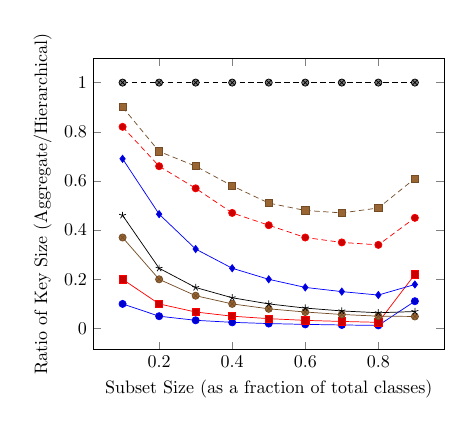
\begin{tikzpicture}[scale = 0.65]
	 \begin{axis}[
	 		xlabel=Subset Size (as a fraction of total classes),
	 		ylabel=Ratio of Key Size (Aggregate/Hierarchical),
% 	 		nolegend
	 		legend pos={north west}
	 		]
	 \addplot plot coordinates{
	 	(0.1,0.1)
		(0.2,0.05)
		(0.3,0.0333)
		(0.4,0.025)
		(0.5,0.02)
		(0.6,0.0167)
		(0.7,0.0143)
		(0.8,0.0125)
		(0.9,0.111)
	 };
	 %\addlegendentry{$n_1=1$, $n_2=100$}
	 \addplot plot coordinates{
	 	(0.1,0.2)
		(0.2,0.1)
		(0.3,0.067)
		(0.4,0.05)
		(0.5,0.04)
		(0.6,0.033)
		(0.7,0.0287)
		(0.8,0.025)
		(0.9,0.22)
	 };
	 %\addlegendentry{$n_1=2$, $n_2=50$}
	 \addplot plot coordinates{
% 	 0.37	0.2	0.133333	0.1	0.08	0.0666667	0.0571429	0.05	0.0497512
	 	(0.1,0.37)
		(0.2,0.2)
		(0.3,0.1333)
		(0.4,0.1)
		(0.5,0.08)
		(0.6,0.067)
		(0.7,0.057)
		(0.8,0.05)
		(0.9,0.049)
	 };
	 %\addlegendentry{$n_1=4$, $n_2=25$}
	 \addplot plot coordinates{
% 	 0.46	0.245	0.166667	0.125	0.1	0.0833333	0.0714286	0.0640205	0.0685871
	 	(0.1,0.46)
		(0.2,0.245)
		(0.3,0.1667)
		(0.4,0.125)
		(0.5,0.1)
		(0.6,0.083)
		(0.7,0.0714)
		(0.8,0.064)
		(0.9,0.069)
% 		(0.9,0111)
	 };
	 %\addlegendentry{$n_1=5$, $n_2=20$}
	 \addplot plot coordinates{
% 	 0.69	0.465	0.323333	0.245	0.2	0.166667	0.150602	0.135685	0.179211
	 	(0.1,0.69)
		(0.2,0.465)
		(0.3,0.323)
		(0.4,0.245)
		(0.5,0.2)
		(0.6,0.167)
		(0.7,0.150)
		(0.8,0.136)
		(0.9,0.179)
	 };
	 %\addlegendentry{$n_1=10$, $n_2=10$}
% 	 0.82	0.66	0.57	0.467172	0.419565	0.367647	0.34965	0.340136	0.454545
	 \addplot plot coordinates{
	 	(0.1,0.82)
		(0.2,0.66)
		(0.3,0.57)
		(0.4,0.47)
		(0.5,0.42)
		(0.6,0.37)
		(0.7,0.35)
		(0.8,0.34)
		(0.9,0.45)
	 };
	 %\addlegendentry{$n_1=20$, $n_2=5$}
	 \addplot plot coordinates{
% 	 0.9	0.715736	0.656566	0.578534	0.5141	0.481928	0.476654	0.497018	0.617284
	 	(0.1,0.9)
		(0.2,0.72)
		(0.3,0.66)
		(0.4,0.58)
		(0.5,0.51)
		(0.6,0.48)
		(0.7,0.47)
		(0.8,0.49)
		(0.9,0.61)
	 };
	 %\addlegendentry{$n_1=25$, $n_2=4$}
	 \addplot plot coordinates{
	 	(0.1,1)
		(0.2,1)
		(0.3,1)
		(0.4,1)
		(0.5,1)
		(0.6,1)
		(0.7,1)
		(0.8,1)
		(0.9,1)
	 };
	 %\addlegendentry{$(n_1=50$, $n_2=2)$ $\&$ $(n_1=100, n_2=1)$}
	 
	 
\end{axis}
\end{tikzpicture}
\end{subfigure}%
\begin{subfigure}{0.5\textwidth}
\captionsetup{font=scriptsize}
\centering
% \hspace*{1.13 cm}
\includegraphics[scale=0.35]{Figs/Legend.png}
\end{subfigure}
\caption{Key Size ratio - Proposed Aggregate Scheme vs Hierarchical Scheme}
\label{plot:keysize}
\end{figure*}

Next, we compare specifically the key size required for the proposed extended scheme, for different values of $n_1$ and $n_2$ (again corresponding to $n=100$), with that required for a hierarchical encryption construction \cite{sandhu1988cryptographic}. Since our scheme uses a hierarchy depth of $2$, we use the same for the hierarchical construction as well, with $n_1$ nodes in level $0$, and $n_2$ level $1$ nodes in the subtree rooted at each level $0$ node. Figure \ref{plot:keysize} summarizes the findings. Evidently, lower the value of $n_1$, better the key aggregation, hence lower the ratio.

\subsection{Utilization Coefficient Comparison}
\label{subsec:util}

Finally we compare the utilization-coefficient of the extended scheme for various values of $n_1$ and $n_2$ (corresponding to $n=100$) with increase in the number of registered key pairs $l$, where each key pair increases the number of classes by $n_2$. We leave out the configuration $n_1=n,n_2=1$ because that always leads to an utilization coefficient of $1$ but is impractical due to huge space requirements. Figure \ref{fig:util} demonstrates that that beyond a certain value of $l$, the combination $(1,n)$ proposed in \cite{chu2014key} has a lower utilization coefficient that all other combinations of $(n_1,n_2)$ for a given $n$. This emphasizes the advantage of making the choice of $(n_1,n_2)$ flexible.

\begin{figure*}[!t]
\captionsetup{font=scriptsize}
\centering
\begin{subfigure}{0.5\textwidth}
\captionsetup{font=scriptsize}
\centering
% \hspace{100.13cm}
\includegraphics[scale=0.22]{Figs/UtilizationPlot.png}
\end{subfigure}%
\begin{subfigure}{0.5\textwidth}
\captionsetup{font=scriptsize}
\centering
\hspace*{3.13 cm}
\includegraphics[scale=0.3]{Figs/Legend1.png}
\end{subfigure}
\caption{Utilization coefficient vs Newly Registered Keys}
\label{fig:util}
\end{figure*}


\section{Applications of KAC}
\label{sec:applications}

The key-aggregate encryption systems described in this paper are primarily meant for data sharing on the cloud. In this section, we point out some specific applications in which KAC proves to be a very efficient solution.

\subsubsection{Online Collaborative Data Sharing.} The foremost application of KAC is in secure data sharing for collaborative applications. Applications such as Google Drive \cite{googledrive} and Dropbox \cite{dropbox} allow users to share their data on the cloud and delegate access rights to multiple users to specific subsets of their whole data. Even government and corporate organizations require secure data sharing mechanisms for their daily operations. KAC can be easily set up to function on top of standard data sharing applications to provide security and flexibility. Data classes may be viewed as folders containing similar files. The fact that our proposed KAC is identity based means that each folder can have its own unique ID chosen by the data owner. Also, the fact that the ciphertext overhead is only logarithmic in the number of data classes implies that space requirement for any data owner is optimal. Finally, the aggregate key also has low overhead and can be transmitted via a secure channel such as a password protected mail service. Since KAC is easily extensible to multiple data owners, the system is practically deployable for a practical data sharing environment. The other advantage of KAC is that once a system is setup with a set of multilinear maps and public parameters, the same setup with the same set of public parameters can be reused by multiple teams within the same organization. Since data owned by each individual owner is insulated from access by users who do not have the corresponding aggregate key, and each data owner has her own tuple of public, private and authentication keys, a single KAC can support multiple data sharing units, while guaranteeing the same underlying security. This saves the cost of setting up new multilinear maps and public parameters each time. 

\subsubsection{Distribution of Product License and/or Activation Keys.} Suppose a company owns a number of products, and intends to distribute the license files (or activation keys) corresponding to these to different users. The KAC framework allows them to put these keys on the cloud in an encrypted fashion, and distribute an aggregate key corresponding to the license files for multiple products to legally authenticated customers as per their requirements. The legal authentication comes from the fact the user who buys multiple products from the company is given the authentication key and the aggregate key that allows her to decrypt the license file for each product. Since both these keys are of constant size, distributing  these to users is easier than providing a separate license file to each user.

\subsubsection{Patient controlled encryption (PCE).} Patient controlled encryption~(PCE) is a recent concept that has been studied in the literature \cite{benaloh2009patient}. PCE allows a patient to upload her own medical data on the cloud and delegate decryption rights to healthcare personnel as per her requirement. KAC acts as an efficient solution to this problem by allowing patients to define their own hierarchy of medical data and delegate decryption rights to this data to different specialists/medical institutions using aggregate keys in an efficient fashion. Given the multitude of sensitive digital health records existent in today's world, storing this data in local/personal machines is not a viable solution and the cloud seems the best alternative. KAC thus provides a two-way advantage in this regard. Not only does it allow people from across the globe to store their health data efficiently and safely, but also allows them to envisage the support of expert medical care from across the globe. 



\section{A Generalized Basic KAC Construction}
\label{sec:general}

In this section, we present a a generalized basic KAC construction. The essential idea is to run $n_A$ parallel instances of the basic scheme parameterized by $n_B$ number of classes, so that the overall system can handle as many as $n=n_A\times n_B$ data classes. Each of these instances share the same set of public parameters, but use their own set of private and public keys. This leads to a trade-off between the overhead for various system parameters. 

\subsection{The Construction}
\label{subsec:two-tier}

We present the construction for generalized KAC in this section. The construction uses techniques similar to the generalized broadcast encryption scheme proposed in \cite{boneh2005collusion}. The generalization in \cite{boneh2005collusion} trades off the ciphertext size with the public key size. Our scheme, on the other hand, trades off the public parameter size with the public key size and the aggregate key size, while still maintaining constant ciphertext overhead.\\

\noindent \textbf{SetUp}$(1^{\lambda},n_B)$: Randomly pick $\alpha \in \mathbb{Z}_q$. Output the system parameter as $param = (P,Q,Y_{P,\alpha,n_B},Y_{Q,\alpha,n_B}))$. Discard $\alpha$. \\

\noindent \textbf{KeyGen}($n_A$): Randomly pick $\gamma_{1},\cdots,\gamma_{n_A} \in \mathbb{Z}_q$. Let $msk_j=\gamma_j$, $PK^1_j=\gamma_{j}P$ and $PK^2_j=\gamma_{j}Q$ for $1\leq j \leq n_A$. Set the master secret key $msk=(msk_1,\cdots,msk_{n_A})$. Set $PK^1=(PK^1_1,\cdots,PK^1_{n_A})$ and $PK^2=(PK^2_1,\cdots,PK^2_{n_A})$. Finally, set the public key $PK=(PK^1,PK^2)$ and output the tuple $(msk,PK)$.\\

\noindent \textbf{Encrypt}$(PK,i,\mathcal{M})$: Compute $a_i=\lceil i/n_B\rceil$ and $b_i=i \text{ mod } B$. Randomly choose $t\in\mathbb{Z}_q$ and output the ciphertext $\mathcal{C}$ as 
 \begin{equation}
 \mathcal{C}=(c_1,c_2,c_3)=(tQ,t(PK^{2}_{a}+Q_{b}),\mathcal{M}.{e}(P_n,tQ_1)) \nonumber
 \end{equation} 

\noindent \textbf{Extract}$(msk,\mathcal{S})$: For the subset of class indices $\mathcal{S}$ and $1\leq a \leq n_A$, define
\begin{eqnarray}
 \mathcal{S}_{a}&=&\{i|i\in\mathcal{S},\lceil i/n_B\rceil=a\} \nonumber\\
 \mathcal{S}'_a&=&\{b_i=i\text{ mod }n_B|i\in\mathcal{S}_{a}\}\nonumber
\end{eqnarray}
\noindent Next, for $1\leq a \leq n_A$, compute
\begin{equation}
 K^{a}_{\mathcal{S}} = {msk_{a}}\sum_{b\in\mathcal{S}'_a}P_{n+1-b} \nonumber
\end{equation}
\noindent Note that this is indirectly equivalent to setting $K^{a}_{\mathcal{S}}$ to $\sum_{b\in\mathcal{S}'_a}\alpha^{n+1-b}PK^{1}_a$. Finally, output 
\begin{equation}
 K_{\mathcal{S}} = (K^{1}_{\mathcal{S}},\cdots,K^{n_A}_{\mathcal{S}})\nonumber
\end{equation}
\noindent Note that the the aggregate key now consists of $n_A$ elements.\\

\noindent \textbf{Decrypt}$(\mathcal{C},i,K_{\mathcal{S}},\mathcal{S})$: If $i\notin\mathcal{S}$, output $\bot$. Otherwise, compute $a_i=\lceil i/n_B\rceil$ and $b_i=i \text{ mod } B$ and set: 
 \begin{eqnarray} 
 A_{\mathcal{S}}&=&\sum_{(b\in\mathcal{S}'_{a_i},b\neq b_i}P_{n+1-b_i+b} \nonumber \\
 B_{\mathcal{S}}&=&\sum_{(b\in\mathcal{S}'_{a_i}}P_{n+1-b} \nonumber  
 \end{eqnarray} 
 \noindent Return the decrypted message $\hat{\mathcal{M}}$ as:
 \begin{equation}
  \hat{\mathcal{M}}=c_3.\frac{{e}(K^{a_i}_{\mathcal{S}}+A_{\mathcal{S}},c_1)}{{e}(B_{\mathcal{S}},c_2)}\nonumber
 \end{equation} 
\noindent Correctness of the algorithm may be easily proved similarly as in Section \ref{subsec:construction1}. Finally, we note that setting $n_A=1$ and $n_B=n$ gives the basic construction of Section \ref{subsec:construction1}. 


\subsection{Performance and Efficiency}
\label{subsec:perf_twotier}

The choice of $n_A$ and $n_B$ play an important role in system performance. As is clear from the construction, the ciphertext always consists of a constant number of group elements. The public parameter comprises of $n_B$ group elements, while the aggregate key as well as the public key consist of $n_A$ group elements each. Thus choosing a smaller value of $n_B$ is useful for applications requiring low overhead aggregate keys. However, choosing $n_A=n_B=\sqrt{n}$ minimizes overall system overhead combining all parameters.

\textbf{We present the simulation studies with different values of $n_A$ and $n_B$ here}.

% We look at the performance of the general KAC construction from the perspective of both parties involved - the data owner sharing her data and an user accessing the shared data. From the data owner's perspective, each superclass comprises of a basic KAC module parameterized with $n$, with constant size public, private and authentication keys. The encryption process can be speeded up using similar caching techniques described in Section \ref{subsec:perf_basic}. From the user's perspective, the system is an ensemble of basic KAC units - one per superclass. For a user willing to access data from $k$ data owners, the aggregate key and authentication keys have size linear in $k$. It seems difficult to do better than this while maintaining data isolation and privacy for each data owner. As in encryption, the decryption process can also be expedited using appropriate caching techniques. It is important to note that the public $param$, which essentially forms the fundamental basic for the security of the general KAC, is a function of $n$ only, and does not depend on the number of users $M$ registered in the system.
% 
% An important aspect of this construction is to decide on an appropriate value for $n$. Keeping a small $n$ value reduces the size of the public parameter. But then a data owner with a large number of data classes $N$ would have to register with $\lceil N/n \rceil$ public, private and authentication key sets, which may not be desirable. Thus there exists a trade-off in using smaller and larger values of $n$ in this scheme. 

% It is important to note that the security of the system depends on the $(n,n)$-BDHE assumption, as we show next.

% \begin{figure*}
% \centering
% \captionsetup{font=scriptsize}
% \includegraphics[scale=0.4]{Figs/Hierarchical.png}
% \caption{Hierarchical KAC}
% \label{fig:K-tier}
% \end{figure*}

\subsection{Semantic Security of General KAC}
\label{subsec:security_twotier}

For the non-adaptive CPA security of the generalized KAC construction, we state the following theorem.

\begin{Theorem}
\label{th:twotierCPA}
Let $\mathbb{G}_1$ and $\mathbb{G}_2$ be bilinear elliptic curve subgroups of prime order $q$. For any pair of positive integers $n',n (n'>n)$, the generalized KAC is $(\tau,\epsilon,n')$ CPA secure if the asymmetric decision $(\tau,\epsilon,n)$-BDHE assumption holds in $(\mathbb{G}_1,\mathbb{G}_2)$.
\end{Theorem}

\noindent The proof of this theorem is very similar to the proof of Theorem \ref{th:basicCPA} and is hence avoided.

% \noindent{\textit{Proof:}} Let $\mathcal{A}$ be a $\tau$-time adversary such that $|Adv_{\mathcal{A},n'}-\frac{1}{2}| > \epsilon$ for a two-tier KAC system parameterized with a given $n$. We build an algorithm $\mathcal{B}$ that has advantage at least $\epsilon$ in solving the $(n,n)$-BDHE problem in $(\mathbb{G}_1,\mathbb{G}_2)$. Algorithm $\mathcal{B}$ takes as input a random $(n,n)$-BDHE challenge $(I'=(H',P,Q,Y_{P,\alpha,n},Y_{Q,\alpha,n}),Z')$ (where $Z'$ is either ${e}(P_{n+1},H')$ or a random value in $\mathbb{G}_T$), and proceeds as follows.\\
% 
% \noindent \textbf{Init:} $\mathcal{B}$ runs $\mathcal{A}$ and receives the set $\mathcal{S}$ of ciphertext classes that $\mathcal{A}$ wishes to be challenged on. $\mathcal{B}$ then randomly chooses a ciphertext class $(a,b)\in\mathcal{S}$.\\
% 
% \noindent \textbf{SetUp}: As discussed before, $\mathcal{B}$ should generate the public $param$, public key $PK$, the authentication key $U$, and the aggregate key $K_{\overline{\mathcal{S}}}$ and provide them to $\mathcal{A}$. They are generated as follows.
% %  \vspace{-0.6mm}
%  \begin{itemize}
%   \item $param$ is set as $(P,Q,Y_{P,\alpha,n},Y_{Q,\alpha,n})$.
%   \item $msk^{a}$ is set as some $u$ randomly chosen from $\mathbb{Z}_q$.
%   \item Set $PK^{a}=(PK^{a}_1,PK^{a}_2)$, where $PK^{a}_1$ and $PK^{a}_2$ are computed as $uP - P_{b}$ and $uQ-Q_{b}$ respectively.
%   \item $K^{a}_{\overline{\mathcal{S}}}$ is set as $\sum_{(a,j_2)\notin\mathcal{S}}({u}P_{n+1-j_2}-(P_{n+1-j_2+b}))$.   
%   \item Choose a random $t\in \mathbb{Z}_q$, and set $U^{a}=tQ$.
%  \end{itemize}
%  
% \noindent Since $P$, $Q$ $\alpha$, $U^{a}$ and the $u$ values are chosen uniformly at random, \emph{the public parameters and the public key have an identical distribution to that in the actual construction}. Also note that providing $\mathcal{A}$ with the aggregate key or the authentication key is unnecessary since they do not impart any information about an encrypted message in the class $(a,b)$. \\
% 
% \noindent \textbf{Challenge}: As before, to generate the challenge, $\mathcal{B}$ picks at random two messages $m_0$ and $m_1$ from the set of possible plaintext messages belonging to class $(a,b)$. She randomly picks $b\in\{0,1\}$, and sets the challenge as $(\mathcal{C},m_0,m_1)$, where $\mathcal{C}=(H'-U^{a},uH',m_b.Z')$. We claim that when $Z'={e}(P_{n+1},H')$ (i.e. the input to $\mathcal{B}$ is a valid $(n,n)$-BDHE tuple), then $(\mathcal{C},m_0,m_1)$ is a valid challenge to $\mathcal{A}$ as in a real attack. To see this, we write $H'=t'Q$ for some unknown $t'\in\mathbb{Z}_q$. Then we have $H'-U=rQ$ for some unknown $r=t-t'$, and $uH'$ = $t'(uQ)$ = $t'(uQ-{Q_{b}}+Q_{b})$ = $t'(PK^{a}_2+Q_{b})$. Finally, $m_b.Z'=m_b{e}(P_{n+1},t'Q)$. Thus, by definition, $\mathcal{C}$ is a valid encryption of the message $m_b$ in class $(a,b)$ and hence, $(\mathcal{C},m_0,m_1)$ is a valid challenge to $\mathcal{A}$.\\
% 
% \noindent \textbf{Guess}: The adversary $\mathcal{A}$ outputs a guess $b'$ of $b$. If $b' = b$, $\mathcal{B}$ outputs $0$ (indicating that $Z' = {e}(P_{n+1},H')$). Otherwise, it outputs $1$ (indicating that $Z'$ is a random element in $\mathbb{Z}_T$).\\
%  
% A similar analysis as in Section \ref{subsec:proof_basic} establishes that $\mathcal{B}$ has advantage at least $\epsilon$ in solving the $(n,n)$-BDHE problem in $(\mathbb{G}_1,\mathbb{G}_2)$. This concludes the proof of Theorem \ref{th:twotierCPA}.
% 
% It is important to note that in a practical environment, any data sharing scheme is expected to support a hierarchical organization of data, where different users are given access to different levels of the data. For example, consider an online data pool on the cloud storing an organization's data. The organization (which owns the data) would like to delegate access rights to this data among its employees. Different employees may be given access to different levels of this data depending on their respective credentials and designation. The most common solution to this is to have a pre-defined hierarchical framework for organizing the data, and have keys at different levels of the hierarchy. As pointed out in our previous discussion, highly irregular data access patterns from multiple users could compromise the efficiency of such a hierarchical system by potentially blowing up the size of the key to be shared. Since key aggregation allows us to combine the decryption rights to multiple data classes into a single constant-sized entity, it seems KAC could be the most efficient solution even in this scenario. However, we show next via a small example that the generalized KAC in its original form may not be able to tackle this problem in the most efficient manner.   
% 
% Although the generalized KAC is highly scalable and efficient, it has a drawback in the sense that it fails to support hierarchical organization of data within a single data owner system. Consider the scenario in which a data owner would like to have two distinct folders, namely $F_1$ and $F_2$, that are meant to be accessed by separate user groups. In the generalized KAC framework, she must then have different public, private and authentication keys for these folders. Now if she were to delegate decryption rights to some user for a subset of files both these folders, she would need to provide two aggregate keys, one for each folder. This is because the generalized KAC does not allow her to aggregate these two keys into a single key. If she wants to provide a single aggregate key for both the folders, she would need to have another aggregate system in place to combine these two individual keys. This process is cumbersome and becomes difficult to maintain as the number of hierarchy levels grow. The same disadvantage also persists with the KAC proposed in \cite{chu2014key}. However, since data hierarchy is extremely common in file-based storage systems, we must adopt KAC so as to be able to provide the advantage of key aggregation for any arbitrarily complex hierarchical structure, without the data owner having to worry about the internal details of the aggregation. The modified KAC infrastructure must now support key aggregation at various levels of the hierarchy, while using the same security guarantees provided the fundamental single data owner KAC. This motivates the introduction of an augmented version of the general KAC in the next section, which we refer to as the \emph{hierarchical} KAC.   




% In this section, we focus on building an efficiently extensible version of our proposed scheme that allows an user to economically increase the number of ciphertext classes while registering a new public key-private key pair. We adopt the idea presented in \cite{boneh2005collusion} to develop a hierarchical structure that has multiple instances (say $M$) of the original scheme running in parallel. Each such instance in turn provides \emph{locally aggregate keys} for $n$ ciphertext sub-classes. Each ciphertext class thus now has a double index $(a,b)$ where $1\leq a \leq M$ and $1\leq b \leq n$. This allows the overall setup to handle $n=Mn$ classes. However, it is important to note that all the instances can use the same public parameters. This interaction among the instances helps to largely improve performance. We further point out that while in \cite{boneh2005collusion}, the two-tier construction offers a trade-off between the public parameter size and the ciphertext size, our 
% two-tier scheme actually reduces the public parameter size without compromising on the size of the ciphertext. Further, addition of a single new key increases the number of classes only by $n$ and not by $n$. Setting $n\ll n$ thus achieves significant improvement in performance over the existing proposal.


% \subsection{The Construction of the Two-tier KAC}
% \label{subsec:construction2}
% 
% Let $n$ be a fixed positive integer. Our proposed $n$-two-tier key-aggregate encryption scheme over elliptic curve subgroups is as described below. It may be noted that the bilinear additive elliptic curve sub-group $\mathbb{G}$ and the multiplicative group $\mathbb{G}_T$, as well as the pairing $\hat{e'}$ are the same as in the basic scheme. The algorithm sets up $M=\lfloor n/n\rfloor$ instances of the basic scheme, each of which handles $n$ ciphertext classes. The original scheme is thus a special case of the extended scheme with $M=1$ and $n=n$.
% 
% 
% \begin{enumerate}
%  \item \textbf{Setup}$(1^{\lambda},n)$: Randomly pick $\alpha \in \mathbb{Z}_q$. Compute $P_i$ = ${\alpha^{i}}P \in \mathbb{G}$ for $i = 1,\cdots,n,n+2,\cdots,2n$. Output the system parameter as $param$ = $(P,P_1,\cdots,P_{n},P_{n+2},\cdots,P_{2n})$. The system randomly chooses a secret parameter $t \in \mathbb{Z}_q$ which is not made public. It is only known to data owners with credentials to control client access rights.
%  \item \textbf{Keygen}(): Pick $\gamma_1,\gamma_2,\cdots,\gamma_{M} \in \mathbb{Z}_q$, output the public and master-secret key pair: $PK$=$({pk}_1,pk_{2},\cdots,pk_{M})$=$(\gamma_1P,\gamma_2P,\cdots,\gamma_{M}P)$, and $msk$=$(\gamma_1,\gamma_2,\cdots,\gamma_{M})$.
%  \item \textbf{Encrypt}$(pk_{a},(a,b),m)$: For a message $m \in \mathbb{G}_T$ and an index $(a,b) \in \{1,2,\cdots,M\}\times\{1,2,\cdots,n\}$, randomly choose $r\in\mathbb{Z}_q$ and let $t'=t+r \in\mathbb{Z}_q$. Then compute the ciphertext $\mathcal{C}$=$(rP,t'{(pk_{a}+P_{b})},m.\hat{e'}(P_{n},t'P_1))$ = $(c_1,c_2,c_3)$.
%  \item \textbf{Extract}$(msk=\gamma,\mathcal{S})$: For the set $\mathcal{S}$ of indices $(\hat{a},j_2)$ the aggregate key is computed as $K_{\mathcal{S}}$ = $(k^{1}_{\mathcal{S}},k^{2}_{\mathcal{S}},\cdots,k^{M}_{\mathcal{S}})$, where $k^{i}_{\mathcal{S}}$ = $\sum_{(i,j_2)\in\mathcal{S}}{\gamma_{1}}P_{n+1-j_2}$. The dynamic access control parameter $U$ is computed as $tP$. Thus the net aggregate key is $(K_{\mathcal{S}},U)$ which is transmitted via a secure channel to users that have access rights to $\mathbb{S}$. Note that  $k^{\hat{a}}_{\mathcal{S}}=\sum_{(\hat{a},j_2)\in\mathcal{S}}\alpha^{n+1-j}pk_{\hat{a}}$ for $\hat{a}=1,2,\cdots,M$. 
%  \item \textbf{Decrypt}$(K_{\mathcal{S}}, U, \mathcal{S},(a,b),\mathcal{C}=\{c_1,c_2,c_3\})$: If $(a,b)\notin\mathcal{S}$, output $\bot$. Otherwise return the message $\hat{m}$ = $c_3\frac{\hat{e'}(k^{a}_{\mathcal{S}}+\sum_{(a,j_2)\in\mathcal{S},j_2\neq b}P_{n+1-j_2+b},U+c_1)}{\hat{e'}(\sum_{(a,j_2)\in\mathcal{S}}P_{n+1-j_2},c_2)}$. 
% \end{enumerate}
% 
% The proof of correctness for the two-tier scheme is presented below.
% 
% \begin{scriptsize}
% \begin{equation}
% \begin{split}
%  \hat{m} &= c_3\frac{\hat{e'}(k^{a}_{\mathcal{S}}+\sum_{(a,j_2)\in\mathcal{S},j_2\neq b}P_{n+1-j_2+b},U+c_1)}{\hat{e'}(\sum_{(a,j_2)\in\mathcal{S}}P_{n+1-j_2},c_2)}\\
%   &= c_3\frac{\hat{e'}(\sum_{(a,j_2)\in \mathcal{S}}{\gamma_{a}}P_{n+1-j_2} + \sum_{(a,j_2)\in\mathcal{S},j_2\neq b}P_{n+1-j_2+b},t'P)}{\hat{e'}(\sum_{(a,j_2)\in\mathcal{S}}P_{n+1-j_2},t'(pk_{a}+P_{b})}\\
% %   &= c_3\frac{\hat{e'}(\sum_{(a,j_2)\in \mathcal{S}}{\gamma_{a}}P_{n+1-j_2},t'P)\hat{e'}(\sum_{(a,j_2)\in\mathcal{S}}(P_{n+1-j_2+b})-P_{n+1},t'P)}{\hat{e'}(\sum_{(a,j_2)\in\mathcal{S}}P_{n+1-j_2},t'pk_{a})\hat{e'}(\sum_{(a,j_2)\in\mathcal{S}}P_{n+1-j_2},t'P_{b})}\\
%   &= c_3\frac{\hat{e'}(\sum_{(a,j_2)\in\mathcal{S}}P_{n+1-j_2+b},t'P)}{\hat{e'}(P_{n+1},t'P)\hat{e'}(\sum_{(a,j_2)\in\mathcal{S}}P_{n+1-j_2},t'P_{b})}\\
%   &= c_3\frac{\hat{e'}(\sum_{(a,j_2)\in\mathcal{S}}P_{n+1-j_2+b},t'P)}{\hat{e'}(P_{n+1},t'P)\hat{e'}(\sum_{(a,j_2)\in\mathcal{S}}P_{n+1-j_2+b},t'P)}\\
%   &= m\frac{\hat{e'}(P_{n},t'P_1)}{\hat{e'}(P_{n+1},t'P)}\\
%   &= m
% \end{split}  
% \end{equation}
% \end{scriptsize}
% 
% 
% \subsection{Semantic Security of the Two-tier KAC}
% \label{subsec:proof_general}
% 
% \subsubsection{The Reduced Two-tier Scheme:}
% 
% We define a reduced version of the two-tier encryption scheme. We note that the ciphertext $\mathcal{C}=(c_1,c_2,c_3)$ output by the $Encypt$ operation essentially embeds the value of $m$ in $c_3$ by multiplying it with $\hat{e'}(P_{n},tP_1)$. Consequently, the security of our proposed scheme is equivalent to that of a \emph{reduced} two-tier key-aggregate encryption scheme that simply uses the reduced ciphertext $(c_1,c_2)$, the aggregate key $K_{\mathcal{S}}$ and the dynamic access parameter $U$ to successfully transmit and decrypt the value of $\hat{e'}(P_{n},t'P_1)=\hat{e'}(P_{n+1},t'P)$. We prove the semantic security of this \emph{reduced scheme} parameterized with a given number of ciphertext classes $n$ for each instance, which also amounts to proving the semantic security of our original encryption scheme for the same number of ciphertext classes. Note that the proof of security is independent of the number of instances $M$ that run in parallel.
% 
% \subsubsection{The Adversarial Model:} We make the following assumptions about the adversary $\mathcal{A}$:
% 
% \begin{enumerate}
%  \item The adversary has the aggregate key that allows her to access any ciphertext class other than those in the target subset $\mathcal{S}$, that is, she possesses $K_{\overline{\mathcal{S}}}$.
%  \item The adversary has access to the public parameters $param$ and $PK$, and also possesses the dynamic access parameter $U$.
% %  \item The adversary is authorized and and hence 
% \end{enumerate}
% 
% 
% \subsubsection{The Security Proof:}
% 
% The security proof presented here uses the first complexity assumption stated in \ref{subsubsec:asm_1}. Let $\mathbb{G}$ be a bilinear elliptic curve subgroup of prime order $q$. For any pair of positive integers $n,n' (n'>n)$ our proposed $n$-two-tier reduced key-aggregate encryption scheme over elliptic curve subgroups is $(\tau,\epsilon,n')$ semantically secure if the decision $(\tau,\epsilon,n)$-BDHE assumption holds in $\mathbb{G}$. We now prove this statement below.
% 
% \textbf{\noindent{Proof:}} Let for a given input $n'$, $\mathcal{A}$ be a $\tau$-time adversary that has advantage greater than $\epsilon$ for the \emph{reduced scheme} parameterized with a given $n$. We build an algorithm $\mathcal{B}$ that has advantage at least $\epsilon$ in solving the $n$-BDHE problem in $\mathbb{G}$. Algorithm $\mathcal{B}$ takes as input a random $n$-BDHE challenge $(P,H,Y_{(P,\alpha,n)},Z)$ where $Z$ is either $\hat{e'}(P_{n+1},H)$ or a random value in $\mathbb{G}_T$. Algorithm $\mathcal{B}$ proceeds as follows.
% 
% \begin{enumerate}
%  \item \textbf{Init:} Algorithm $\mathcal{B}$ runs $\mathcal{A}$ and receives the set $\mathcal{S}$ of ciphertext classes that $\mathcal{A}$ wishes to be challenged on. For each ciphertext class $(a,b)\in\mathcal{S}$, $\mathcal{B}$ performs the \textbf{SetUp}-$\mathbf{(a,b)}$, \textbf{Challenge}-$\mathbf{(a,b)}$ and \textbf{Guess}-$\mathbf{(a,b)}$ steps. Note that the number of iterations is polynomial in $|S|$. 
%  
%  \item \textbf{SetUp}-$\mathbf{(a,b)}$: $\mathcal{B}$ should generate the public $param$, public key $PK$, the access parameter $U$, and the aggregate key $K_{\overline{\mathcal{S}}}$. For the iteration corresponding to ciphertext class $(a,b)$, they are generated as follows.
%  \begin{itemize}
%   \item $param$ is set as $(P,Y_{P,\alpha,n})$.
%   \item Randomly generate $u_1,u_2,\cdots,u_{M} \in \mathbb{Z}_q$. Then, set $PK$= $(pk_1,pk_2,\cdots,pk_{M})$, with $pk_{\hat{a}}$ = $u_{\hat{a}}P - P_{b}$ for $\hat{a}=1,2,\cdots,M$.
%   \item Set $K_{\overline{\mathcal{S}}}$ = $(k^{1}_{\overline{\mathcal{S}}},k^{2}_{\overline{\mathcal{S}}},\cdots,k^{M}_{\overline{\mathcal{S}}})$, where $k^{\hat{a}}_{\overline{\mathcal{S}}}$ is set as $\sum_{(\hat{a},j_2)\notin\mathcal{S}}({u_{\hat{a}}}P_{n+1-j_2}-(P_{n+1-j_2+b}))$. Then, $k^{\hat{a}}_{\overline{\mathcal{S}}}$ = $\sum_{(\hat{a},j_2)\notin\mathcal{S}}\alpha^{n+1-j_2}pk_{\hat{a}}$,which is as per the scheme specification. Note that $\mathcal{B}$ knows that $(a,b)\notin \overline{\mathcal{S}}$, and hence has all the resources to compute this aggregate key for $\overline{\mathcal{S}}$. 
%   \item $U$ is set as some random element in $\mathbb{G}$.
%  \end{itemize}
%  
%  Note that since $P$, $\alpha$, $U$ and the $u_{\hat{a}}$ values are chosen uniformly at random, the public key has an identical distribution to that in the actual construction.
%  
%  \item \textbf{Challenge}-$\mathbf{(a,b)}$: To generate the challenge for the ciphertext class $(a,b)$, $\mathcal{B}$ computes $(c_1,c_2)$ as $(H-U,u_{a}H)$. It then randomly chooses a bit $b\in{(0,1)}$ and sets $K_b$ as $Z$ and $K_{1-b}$ as a random element in $\mathbb{G}_T$. The challenge given to $\mathcal{A}$ is $((c_1,c_2),K_0,K_1)$. 
%  
%  We claim that when $Z=\hat{e'}(P_{n+1},H)$ (i.e. the input to $\mathcal{B}$ is a $n$-BDHE tuple), then $((c_1,c_2),K_0,K_1)$ is a valid challenge to $A$. We prove this claim here. we point out that $P$ is a generator of $\mathbb{G}$ and so $H=t'P$ for some $t'\in\mathbb{Z}_q$. Putting $H$ as $t'P$ gives us the following:
%  \begin{itemize}
%   \item  $U=tP$ for some $t\in\mathbb{Z}_q$
%   \item $c_1=H-U=(t'-t)P=rP$ for $r=t'-t$
%   \item $c_2=u_{a}H=(u_{a})t'P=t'(u_{a}P)=t'(u_{a}P-P_{b}+P_{b})=t'(pk_{a}+P_{b})$
%   \item $K_b=Z=\hat{e'}(P_{n+1},H)=\hat{e'}(P_{n+1},t'P)$
%  \end{itemize}
%  On the other hand, if $Z$ is a random element in $\mathbb{G}_T$ (i.e. the input to $\mathcal{B}$ is a random tuple), then $K_0$ and $K_1$ are just random independent elements of $\mathbb{G}_T$.
%  
%  \item\textbf{Guess}-$\mathbf{(a,b)}$: The adversary $\mathcal{A}$ outputs a guess $b'$ of $b$. If $b' = b$, $\mathcal{B}$ outputs $0$ (indicating that $Z = \hat{e'}(P_{n+1},H)$), and terminates. Otherwise, it goes for the next ciphertext class in $\mathcal{S}$.
% \end{enumerate}
% If after $|\mathcal{S}|$ iterations, $b' \neq b$ for each ciphertext class $(a,b)\in\mathcal{S}$, the algorithm $\mathcal{B}$ outputs $1$ (indicating that $Z$ is random in $\mathbb{G}_T$). We now analyze the probability that $\mathcal{B}$ gives a correct output. If $(P,H,Y_{(P,\alpha,n)},Z)$ is sampled from $R$-BDHE, $Pr[\mathcal{B}(G,H,Y_{(P,\alpha,n)},Z)=0]$ = $\frac{1}{2}$, while if $(P,H,Y_{(P,\alpha,n)},Z)$ is sampled from $L$-BDHE, $|Pr[\mathcal{B}(G,H,Y_{(P,\alpha,n)},Z)]-\frac{1}{2}|$ $\geq$ $\epsilon$. So, the probability that $\mathcal{B}$ outputs correctly is at least $1-(\frac{1}{2}-\epsilon)^{|\mathcal{S}|} \geq \frac{1}{2}+\epsilon$. Thus $\mathcal{B}$ has advantage at least $\epsilon$ in solving the $n$-BDHE problem. This concludes the proof. \emph{Note that the instance of this proof with $M=1$ and $n=n$ serves as the proof of security for the basic KAC scheme proposed in Section \ref{sec:proposal}}.
% 
% 
% \subsubsection{Performance Trade off with the Basic Scheme:} 
% 
% We compare the various parameter sizes for the proposed original and extended schemes in table \ref{tab:tradeoff}. We note that $SetUp$ and $KeyGen$ are both one-time operations, and for a given subset $\mathcal{S}$, the $Extract$ operation is also performed once to generate the corresponding aggregate key $K_{\mathcal{S}}$. The most important advantage that the two-tier scheme provides is the user's ability to efficiently extend the number of ciphertext classes. As far as encryption and decryption are concerned, encryption should ideally take the same time for both schemes, while decryption is actually expected to be faster for the two-tier construction as $n\leq n$.  
% 
% \begin{table}[!t]
% \captionsetup{font=scriptsize}
% \caption{Comparison between the Basic and Two-tier schemes}
% \label{tab:tradeoff}
% \begin{center}
% \scalebox{0.75}{
% \begin{tabular}{|c|c|c|c|}
% 
% %Symbol & Fault Model \\
% %(MHz)&$\ $ &$\ $ & $\ $\\
% \hline
% \textbf{Item} & \textbf{Nature of Computation} & \textbf{Original scheme} & \textbf{Two-tier scheme}\\\hline\hline
% 
% $param$(SetUp) & One-time & $\mathcal{O}(n)$ & $\mathcal{O}(n)$\\\hline
% $PK$(KeyGen) & One-time &$\mathcal{O}(1)$ & $\mathcal{O}(M)$\\\hline
% $K_{\mathcal{S}}$(Extract) & One-time & $\mathcal{O}(1)$ & $\mathcal{O}(M)$\\\hline
% $\mathcal{C}$ & One per Message & $\mathcal{O}(1)$ & $\mathcal{O}(1)$\\\hline
% Encrypt & One Per Message & $\mathcal{O}(1)$ & $\mathcal{O}(1)$\\\hline
% Decrypt & One Per Message & $\mathcal{O}(|\mathcal{S}|)$ & $\mathcal{O}(|\mathcal{S}|)$\\\hline
% % Ciphertext Class Extension & Dynamic & Not Possible & $\mathcal{O}(n)$\\\hline
% \hline
% % OSB & Other Single Byte Faults (More than 4 bits in one byte affected)  \\
% % MB & Multiple Byte Faults  \\
% 
% % \hline \hline
% \end{tabular}
% }
% 
% \end{center}
% \end{table}
% 
% 
% \subsection{A Flexible Extension Policy}
% \label{subsec:extension}
% 
% If a user needs to classify her ciphertexts into more that $n$ classes, she can register for additional key pairs $(pk_{M+1},msk_{M+1})$, $\cdots$, $(pk_{M+l},msk_{M+l})$ as per her requirements. Each new key registration increases the number of classes by $n$, where $n\leq n$. The idea of under-utilization stems from the fact that registration of each public-private key pair increases the number of classes by $n$. However, it is not necessary that all the existing classes are utilized at any given point of time. For instance, a user may at any point of time want to register $l$ new private-public key pairs, however she will in all probability not use up all $ln$ additional classes of messages that could be encrypted using the newly registered keys. We stress here is that, unlike in the public key extension scheme proposed in \cite{chu2014key} where the values of $M$ and $n$ are fixed to $1$ and $n$ respectively, our two-tier construction \emph{provides a choice} of $M$ and $n$ so that the system administrator could choose pair of values suited to their requirements. 
% 
% We propose a metric to quantify the under-utilization of ciphertext classes for a given configuration of the system. Let us assume that at some instance of time, there are $M+l$ private-public key pairs registered in the system, and $c_i$ classes corresponding to each key are being utilized. We define the utilization coefficient as $\frac{1}{1+\xi}$, where $\xi=-\frac{1}{M}\sum_{i=1\\c_i\neq0}^{M}\log(\frac{c_i}{n})$. An efficient scheme tries to minimize the value of $\xi$ to achieve good utilization of the existing set of classes. The value is maximum when $c_i=n \forall i=1,2,\cdots,n$. Note that $c_i=0$ implies that no subclasses under the given key $pk_i$ are being utilized, which is equivalent to not registering the key at all.        
% 
% 
% To stress the importance of the flexible extension policy, we provide a simplified example here. We consider two possible configurations of the extended scheme. In the first configuration, $M=1$ and $n=n$, which is essentially identical to the public key extension scheme proposed in \cite{chu2014key}. The other configuration has $M>1$ and $n<n$. Now assume that before extension, both schemes utilized $c$ ciphertext classes out of the $n$ possible classes, equally distributed across all key pairs. Now suppose a situation arises where an user needs to register $l$ more key pairs, and utilizes $z<n$ classes corresponding to each key. In the first configuration, we have $\xa=-\frac{1}{l+1}(l\log(\frac{z}{n})+\log(\frac{c}{n}))$, while for the second configuration, $\xb=-\frac{1}{l+M}(l(\log(\frac{z}{n}))+M\log(\frac{c}{n}))$. Now for $l>(\frac{M}{\log M}-1)\log(\frac{z}{c})-1$, $\xb<\xa$. Thus for any value of $(M,n)$ other than $(1,n)$, there exists a value of $l$ for which the 
% scheme achieves better utilization coefficient. Since $l$ is expected to increase in a dynamic scenario, our public key extension scheme eventually performs better than the scheme suggested in \cite{chu2014key}. 
% 
% \subsection{Advantage over Hierarchical Encryption Based Schemes}
% \label{subsec:advantage}
% 
% \begin{figure}[!t]
% \centering
% \captionsetup{font=scriptsize}
% \includegraphics[scale=0.4]{Figs/tree.png}
% \caption{A Practical Request Scenario in the Hierarchical Setting}
% \label{fig:agg}
% \end{figure}
% 
% Although the two-tier scheme has a two level hierarchy (with each of the $M$ parallely executing instances of the basic scheme representing a node in the top level and the actual ciphertext classes representing nodes in the lower level), it avoids the pitfalls of existing hierarchical encryption based schemes \cite{akl1983cryptographic,ateniese2012provably}. In standard tree based hierarchical systems, granting access to the key corresponding to any node implicitly grants access to all the keys in the subtree rooted at that node. This means granting access to a selected set of nodes in a given subtree would blow up the key-size to be the same as the number of nodes. This is avoided in our two-tier scheme, since any number of nodes (ciphertext classes) that belong to the same instance may be aggregated into a single key. Figure \ref{fig:agg} summarizes this phenomenon. In the situation depicted, a tree-based hierarchy system would require $4$ decryption keys, while our 
% scheme would require only $2$. In this respect, our scheme has similar advantages to that of \cite{chu2014key}.
% 
% 
% 
% 
% 
% 
% 
% 
% 
% 
% 

\section{Chosen Ciphertext Secure Basic KAC}
\label{sec:CCA}

We now demonstrate how to modify the basic KAC proposed in Section \ref{subsec:construction1} to obtain chosen ciphertext security. The resulting KAC system is proven to be CCA secure in the standard model without using random oracles. To the best of our knowledge, this is the first CCA secure KAC proposed in the cryptographic literature.

\subsection{Additional Requirements for CCA Security}
\label{subsec:additional}

We have the following additional requirements for the CCA secure basic KAC:

\begin{itemize}
 \item A signature scheme $(SigKeyGen,Sign,Verify)$. 
 \item A collision resistant hash function for mapping verification keys to $\mathbb{Z}_q$. 
\end{itemize}

For simplicity of presentation, we assume here that the signature verification keys are encoded as elements of $\mathbb{Z}_q$. We avoid any further mention of the hash function in the forthcoming discussion, since it is implicitly assumed that any signature value we refer to is essentially the hash value corresponding to the original signature.

\subsection{Construction}
\label{subsec:construction_CCA}

We will demonstrate in the following section that the security of CCA-secure Dynamic KAC for $n$ data classes is based on the asymmetric $(n+1)$-BDHE assumption, instead of the asymmetric $n$-BDHE assumption as for the basic scheme. For consistency of notation, we describe here the CCA-secure dynamic KAC for $n-1$ users, such that the security assumption is still the asymmetric $n$-BDHE assumption as before. \\

% \begin{enumerate}
 \noindent \textbf{SetUp}$(1^{\lambda},n-1)$: Randomly pick $\alpha \in \mathbb{Z}_q$. Output the system parameter as $param = (P,Q,Y_{P,\alpha,n},Y_{Q,\alpha,n}))$. Discard $\alpha$.
 
 \noindent \textbf{KeyGen}(): Same as in the basic scheme of Section \ref{subsec:construction1}.\\
 
 \noindent \textbf{Encrypt}$(PK,i,\mathcal{M})$: Run the $SigKeyGen$ algorithm to obtain a signature signing key $K_{SIG}$ and a verification key $V_{SIG} \in \mathbb{Z}_q$. Then, randomly choose $t\in\mathbb{Z}_q$ and set 
 \begin{eqnarray}
 c_0=tQ&\text{and}& c_1 = t{(PK_2+Q_i+V_{SIG}Q_n)}\nonumber\\
 c_2 &=& \mathcal{M}.{e}(P_n,tQ_1)\nonumber\\
 \mathcal{C}&=&((c_0,c_1,c_2),Sign(\mathcal{C}',K_{SIG}),V_{SIG}) \nonumber
 \end{eqnarray}
 \noindent Output the ciphertext $\mathcal{C}$.\\
 
 \noindent \textbf{Extract}$(msk,\mathcal{S})$: Same as in Section \ref{subsec:construction1}.\\
 
 \noindent \textbf{Decrypt}$(\mathcal{C},i,\mathcal{S},K_{\mathcal{S}})$: Let $\mathcal{C}=(\mathcal{C}',\sigma,V_{SIG})$. Verify that $\sigma$ is a valid signature of $\mathcal{C}'$ under the key $V_{SIG}$. If not, output $\bot$. Also, if $i\notin\mathcal{S}$, output $\bot$. Otherwise, pick a random $w\in \mathbb{Z}_q$ and set 
 \begin{eqnarray}
  SIG_{\mathcal{S}} &=& \sum_{j\in\mathcal{S}}V_{SIG}P_{2n+1-j}\nonumber\\
  a_{\mathcal{S}} &=& \sum_{j\in\mathcal{S},j\neq i}P_{n+1-j+i}\nonumber\\
  b_{\mathcal{S}} &=& \sum_{j\in\mathcal{S}}P_{n+1-j}\nonumber  
 \end{eqnarray}
 \noindent Note that these can be computed as $1\leq i,j \leq n-1$. Next, set two entities $\hat{h}_1$ and $\hat{h}_2$ as
 \begin{eqnarray}
  \hat{h}_1 &=& K_{\mathcal{S}} + SIG_{\mathcal{S}} + a_{\mathcal{S}} + w(PK_1+P_i+V_{SIG}P_n)\nonumber\\
  \hat{h}_2 &=& b_{\mathcal{S}}+wP \nonumber
 \end{eqnarray}
 \noindent Output the decrypted message 
 \begin{equation}
  \hat{\mathcal{M}} = c_2\frac{{e}(\hat{h}_1,c_0)}{{e}(\hat{h}_2,c_1)}\nonumber
 \end{equation}
\noindent The proof of correctness of this scheme is very similar to the proof for the basic dynamic KAC scheme presented in Section \ref{subsec:construction1}. Note that the ciphertext size is still constant and everything else, including the public and private parameters, as well as the aggregate key, remains unchanged. The main change from the original scheme is in the fact that decryption requires a randomization value $w\in\mathbb{Z}_q$. This randomization makes sure that that the pair $(\hat{h}_1,\hat{h}_2)$ is chosen from the following distribution 
\begin{equation}
(x(PK_1+P_i+V_{SIG}P_n)-P_{n+1},xP) \noindent
\end{equation}
\noindent where $x$ is chosen uniformly from $\mathbb{Z}_q$. To verify this claim, set $x=w+\sum_{j\in\mathcal{S}}\alpha^{n+1-j}$. Moreover, since $w$ is uniformly random in $\mathbb{Z}_q$, so is $x$. \emph{This randomization is a vital aspect from the point of view of CCA-security}. Note that the distribution $(\hat{h}_1,\hat{h}_2)$ depends on the ciphertext class $i$ for the message $m$ to be decrypted. 



 
\subsection{Proof of CCA-Security}
\label{subsec:proof_cca}

We begin by recalling that a signature scheme $(SigKeyGen,Sign,Verify)$ is said to be $(\tau,\epsilon,q_S)$ strongly existentially unforgeable if no $\tau$-time adversary, making at most $q_{S}$ signature signature queries, fails to produce some new message-signature pair with probability at least $\epsilon$. For a more complete description, refer \cite{canetti2004chosen}.

\begin{Theorem}
\label{th:basicCCA}
Let $\mathbb{G}_1$ and $\mathbb{G}_2$ be bilinear elliptic curve subgroups of prime order $q$. For any positive integer $n$, the modified basic KAC is $(\tau,\epsilon_1+\epsilon_2,n-1,q_D)$ CCA-secure if the decision $(\tau,\epsilon,n,n)$-BDHE assumption holds in $(\mathbb{G}_1,\mathbb{G}_2)$ and the signature scheme is $(t,\epsilon_2,1)$ strongly existentially unforgeable.
\end{Theorem}

\noindent{\textit{Proof:}} Let $\mathcal{A}$ be a $\tau$-time adversary such that $|Adv_{\mathcal{A},n-1}-\frac{1}{2}|$ $>$  $\epsilon_1+\epsilon_2$. We build an algorithm $\mathcal{B}$ that has advantage at least $\epsilon_1$ in solving the asymmetric $n$-BDHE problem in $\mathbb{G}$. Algorithm $\mathcal{B}$ takes as input a random asymmetric $n$-BDHE challenge $(I=(H,P,Q,Y_{P,\alpha,l},Y_{Q,\alpha,l}),Z)$ (where $Z$ is either ${e}(P_{n+1},H)$ or a random value in $\mathbb{G}_T$), and proceeds as follows.\\

\noindent\textbf{Init:} $\mathcal{B}$ runs $\mathcal{A}$ and receives the set ${\mathcal{S}}^{*}$ of ciphertext classes that $\mathcal{A}$ wishes to be challenged on. $\mathcal{B}$ then randomly chooses a ciphertext class $i\in{\mathcal{S}}^{*}$.\\
 
\noindent\textbf{SetUp}: $\mathcal{B}$ should generate the public $param$, public key $PK$, the authentication key $U$, and the aggregate key $K_{\overline{{\mathcal{S}}^{*}}}$, and provide them to $\mathcal{A}$. Algorithm $\mathcal{B}$ first runs the $SigKeyGen$ algorithm to obtain a signature signing key ${K^{*}_{SIG}}$ and a corresponding verification key ${V^{*}_{SIG}} \in \mathbb{Z}_q$. $\mathcal{B}$ generates the following:
%  \vspace{-0.6mm}
 \begin{itemize}
  \item $param$ is set as $(P,Q,Y_{P,\alpha,n},Y_{Q,\alpha,n})$.
  \item Set $PK=(PK_1,PK_2)$, where $PK_1$ and $PK_2$ are computed as $\gamma P - {V^{*}_{SIG}}P_n - P_i$ and $\gamma Q - {V^{*}_{SIG}}Q_n - Q_i$ respectively for $\gamma$ chosen uniformly at random from $\mathbb{Z}_q$. Note that this is equivalent to setting $msk=\gamma-\alpha^{i}-\alpha^{n}{V^{*}_{SIG}}$.
  \end{itemize}
  \noindent $\mathcal{B}$ computes the collusion aggregate key $K_{\overline{{\mathcal{S}}^{*}}}$ as 
  \begin{equation}
   K_{\overline{{\mathcal{S}}^{*}}} = \sum_{j\notin{\mathcal{S}}^{*}}({u}P_{n+1-j}- {V^{*}_{SIG}}P_{2n+1-j} -P_{n+1-j+i}) \nonumber
  \end{equation}  
\noindent Note that $K_{\overline{{\mathcal{S}}^{*}}}$ is equal to $\sum_{j\notin{\mathcal{S}}^{*}}\alpha^{n+1-j}PK_1$, in accordance with the specification provided by the scheme. Moreover, $\mathcal{B}$ is aware that $i\notin \overline{{\mathcal{S}}^{*}}$ (implying $i\neq j$). Also, $j\neq n$ as $1\leq j \leq n-1$. Hence, $\mathcal{B}$ has all the resources to compute $K_{\overline{{\mathcal{S}}^{*}}}$.

Since $P$, $Q$, $\alpha$, and $\gamma$ are chosen uniformly at random, \emph{the public parameters and the public key have an identical distribution to that in the actual construction}.\\
 
\noindent\textbf{Query Phase 1}: Algorithm $\mathcal{A}$ now issues decryption queries. Let $(j,\mathcal{C})$ be a decryption query where $j\in{\mathcal{S}}^{*}$. Let $\mathcal{C}=((c_0,c_1,c_2),\sigma,V_{SIG})$. Algorithm $\mathcal{B}$ first runs $Verify$ to check if the signature $\sigma$ is valid on $(c_0,c_1,c_2)$ using $V_{SIG}$. If invalid, $\mathcal{B}$ returns $\bot$. If $V_{SIG} = {V^{*}_{SIG}}$, $\mathcal{B}$ outputs a random bit $b\in\{0,1\}$ and \emph{aborts} the simulation. Otherwise, the challenger picks a random $x\in\mathbb{Z}_q$. It then sets
\begin{eqnarray}
 \hat{h}_0&=&(V_{SIG}-{V^{*}_{SIG}})P_n+P_j-P_i\nonumber\\
 \hat{h'}_0&=&{(V_{SIG}-{V^{*}_{SIG}})}^{-1}(P_{j+1}-P_{i+1})\nonumber \\
 \hat{h}_2&=&xP+{(V_{SIG}-{V^{*}_{SIG}})}^{-1}P_1\nonumber\\
 \hat{h}_1&=&u\hat{h}_2 + xd_0 + d'_0 \nonumber 
\end{eqnarray}
\noindent $\mathcal{B}$ responds with $K=c_2\frac{{e}(\hat{h}_1,c_0)}{{e}(\hat{h}_2,c_1)}$. To see that this response is as in a real attack game, set $x'=x+\alpha{(V_{SIG}-{V^{*}_{SIG}})}^{-1}$ and observe that $\hat{h}_2$ = $x'P$ and $\hat{h}_1$ = $x'(PK_1+P_i+V_{SIG}P_n)-P_{n+1}$. Furthermore, since $x$ is uniform in $\mathbb{Z}_q$, $x'$ is also uniform in $\mathbb{Z}_q$. Thus, $\mathcal{B}$'s response is a valid decryption as required.\\
 
\noindent\textbf{Challenge}:To generate the challenge, $\mathcal{B}$ picks at random two messages $\mathcal{M}_0$ and $\mathcal{M}_1$ from the set of possible plaintext messages belonging to class $i$. She randomly picks $b\in\{0,1\}$, and sets 
\begin{eqnarray}
 \mathcal{C}&=&(H,\gamma H,\mathcal{M}_b.Z)\nonumber\\
 \mathcal{C}^{*}&=&(\mathcal{C},Sign(\mathcal{C},{K^{*}_{SIG}}),{V^{*}_{SIG}})\nonumber
\end{eqnarray}
\noindent The challenge posed to $\mathcal{A}$ is $(\mathcal{C}^{*},\mathcal{M}_0,\mathcal{M}_1)$. It is easy to show that when $Z={e}(P_{n+1},H)$, $({\mathcal{C}}^{*},\mathcal{M}_0,\mathcal{M}_1)$ is a valid challenge to $\mathcal{A}$ as in a real attack.\\
 
\noindent\textbf{Query Phase 2}: Same as in Query Phase 1.\\ 
 
\noindent\textbf{Guess}: The adversary $\mathcal{A}$ outputs a guess $b'$ of $b$. If $b' = b$, $\mathcal{B}$ outputs $0$. Otherwise, it outputs $1$.\\

\noindent Quite evidently, if $(I,Z)$ is sampled from ${\mathcal{R}'}_{\text{BDHE}}$, $Pr[\mathcal{B}(I,Z)=0]$ = $\frac{1}{2}$. Let \textbf{abort} be the event that $\mathcal{B}$ aborted the simulation. Now when $(I,Z)$ is sampled from ${\mathcal{L}'}_{\text{BDHE}}$, we have 
\begin{equation}
 |Pr[\mathcal{B}(I,Z)]-\frac{1}{2}|>(\epsilon_1+\epsilon_2)-Pr[\textbf{abort}] \nonumber
\end{equation}
\noindent This essentially implies that $\mathcal{B}$ has advantage at least $\epsilon_1+\epsilon_2-Pr[\text{\textbf{abort}}]$ in solving the asymmetric $n$-BDHE problem in $(\mathbb{G}_1,\mathbb{G}_2)$.\\


\noindent We now bound the probability that $\mathcal{B}$ aborts the simulation as a result of one of the decryption queries by $\mathcal{A}$. We claim that $Pr[\textbf{abort}]<\epsilon_2$; otherwise one can use $\mathcal{A}$ to forge signatures with probability at least $\epsilon_2$. A very brief proof of this may be stated as follows. We may construct a simulator that knows the master secret key $u$ and receives ${K^{*}_{SIG}}$ as a challenge in an existential forgery game. $\mathcal{A}$ can then cause an abort by producing a query that leads to an existential forgery under ${K^{*}_{SIG}}$ on some ciphertext. Our simulator uses this forgery to win the existential forgery game. Only one chosen message query is made by the adversary during the game to generate the signature corresponding to the challenge ciphertext. Thus, $Pr[\text{abort}]<\epsilon_2$, implying $\mathcal{B}$ has advantage at least $\epsilon_1$ in solving the asymmetric $n$-BDHE problem in $(\mathbb{G}_1,\mathbb{G}_2)$. This completes the proof of Theorem \ref{th:basicCCA}.\hfill\qed 

The extended KAC construction for multiple users presented in Section \ref{sec:extendedconstruction}, as well the generalized basic KAC construction from Section \ref{sec:general} may also be similarly modified to obtain CCA security.  






% \input{Source_TDSC/Hierarchical}


\section{Conclusions}
\label{sec:conclusions}

To be Written

\begin{scriptsize}
\bibliographystyle{unsrt}
\bibliography{bib/KeyAggregate}
\end{scriptsize}

% \newpage
% \appendix


% % However, KAC suffers from the following major drawbacks:
% % 
% % \begin{enumerate}
% %  \item KAC uses bilinear non-degenerate pairings over multiplicative groups. Recent reports from NIST \cite{NIST2009} have demonstrated that the security of RSA over multiplicative cyclic groups for a key size of $1024$ bits has the same security as RSA over additive elliptic curve groups with a key size of $160$ bits. Thus defining KAC over multiplicative groups is possibly not the most computationally efficient scheme; an adaptation of the scheme to additive elliptic curve group would certainly be more efficient.
% %  \item KAC is a static scheme in the sense that once a user is in possession of the aggregate key corresponding to a subset of files from data owner, the owner cannot dynamically revoke the permission of the client for accessing one or more updated files. Since dynamic changes in access rights is extremely common in shared data storage on cloud, this scenario needs to be tackled. 
% %  \item The public key extension of KAC proposed in \cite{chu2014key} is extremely cumbersome and resource consuming since registration of each new public key-private key pair requires the number of classes to be extended by th original number of classes.
% %  \end{enumerate}
% 
% % In this work, we aim to scheme for online data sharing that overcomes to a large extent all of the above mentioned drawbacks of KAC.
% 
% % In this paper we aim to present a scheme the above drawbacks of KAC. We also present security proofs for our proposed scheme. We then further extend the scheme using the ideas presented in \cite{} to make it secure against chosen ciphertext attacks.
% 
% 
% 
% 
% \section{Bilinear Maps and the BDHE on Elliptic Curves}
% \label{app_sec:prelims}
% 
% \subsection{Bilinear Pairings}
% 
% We  present a brief outline of the necessary facts about bilinear pairings on elliptic curves that are used in the forthcoming discussion. Let $\mathbb{K}=F_{p}$ be a field of prime order $p$, and let an elliptic curve over $\mathbb{K}$ be defined by the Weierstrass \cite{miller1986use} equation:
% \begin{equation*}
%  E(\mathbb{K}) : y^2 + a_1xy + a_3y = x^3 + a_2x^2 + a_4x + a_6
% \end{equation*}
% 
% where $a_1, a_2, a_3, a_4, a_5 \in \mathbb{K}$. The curve must be non-singular. In particular, if $char(\mathbb{K})\neq2,3$, the equation takes the special form $y^2=x^3+a_4x+a_6$ with $4{a_4}^3+27{a_6}^2\neq0$. Let $\overline{K} = F_{p^k}$ be the smallest extension field of $K=F_p$ that contains the $q^{th}$ roots of unity. Here, $k$ is called the embedding degree with respect to $K$ and $q$. We denote the set of $q$-torsion points on the elliptic curve as $E(\overline{K})[q]$ ($q$-torsion points essentially have order $q$).
% 
% A pairing is a bilinear map defined over elliptic curve subgroups. Let $\mathbb{G}_{1}$ and $\mathbb{G}_{2}$ be two such additive cyclic subgroups of the same prime order $q$ and let $\mathbb{G}_{T}$ be a multiplicative group, also of order $q$ with identity element $1$. Let $P$ and $Q$ be generators for $\mathbb{G}_1$ and $\mathbb{G}_2$ respectively. A pairing $\hat{e'}:\mathbb{G}_1 \times \mathbb{G}_2\longrightarrow\mathbb{G}_T$ satisfying the following the following properties is said to be a bilinear mapping. 
% 
% \begin{itemize}
%  \item Bilinear: $\forall P_1,P_2 \in \mathbb{G}_1, Q_1,Q_2\in\mathbb{G}_2$, and $a,b \in \mathbb{Z}$, we have the following:
%  \begin{eqnarray}
%    \hat{e'}(aP_1,bQ_1) &= \hat{e'}(P_1,Q_1)^{ab}\nonumber\\
%    \hat{e'}(P_1+P_2,Q_1) &= \hat{e'}(P_1,Q_1)\hat{e'}(P_2,Q_1)\nonumber\\
%    \hat{e'}(P_1,Q_1+Q_2) &= \hat{e'}(P_1,Q_1)\hat{e'}(P_1,Q_2)\nonumber
%  \end{eqnarray}
%  \item Non-degeneracy: If for all $P_i \in \mathbb{G}_1, \hat{e'}(P_1,Q_1)=1$ then $Q_1=\mathcal{0}$. Alternatively, if $P$ and $Q$ be the generators for $\mathbb{G}_1$ and $\mathbb{G}_2$ respectively where neither group only contains the point at infinity, then $\hat{e'}(P,Q)\neq1$ 
%  \item Computability: There exists an efficient algorithm to compute $\hat{e'}(R,S)\forall R \in \mathbb{G}_1, S\in\mathbb{G}_2$
% \end{itemize}
% 
% It is important to note that $\mathbb{G}_1$ and $\mathbb{G}_2$ could be identical groups as well.
% 
% % \subsection{The Decisional Bilinear Diffie-Hellman Problem (DBDH)}
% 
% % The three-party Diffie-Hellman key agreement \cite{} lends itself to the decisional form - the decisional bilinear Diffie-Hellman (DBDH) problem. DBDH requires a participant to determine if some target element is either a special combination of given parameters or a random element
% 
% % Let $\mathbb{G}$ be an additive cyclic elliptic curve subgroup of prime order $q$, where $2^{\lambda}\leq q \leq 2^{\lambda + 1}$, such that the point $P$ is a generator for $\mathbb{G}$. Also, let $\mathbb{G}_{T}$ be a multiplicative group of order $q$ with identity element $1$. We assume that there exists an efficiently computable bilinear pairing $\hat{e'}:\mathbb{G} \times \mathbb{G}\longrightarrow\mathbb{G}_T$. The DBDH problem is defined as follows.  Given $aP, bP, cP \in \mathbb{G}$ where $a,b,c\in \mathbb{Z}_q$, and $T\in \mathbb{G}_T$, determine if $T=\hat{e'}(P,P)^{abc}$. 
% 
% % \subsection{The Bilinear Diffie-Hellman Exponent Problem (BDHE)}
% 
% 
% 
% 
% 
% 
% 
% \section{Semantic Security of Key-Aggregate Schemes}
% \label{app_sec:security}
% 
% We now define the semantic security of a key-aggregate encryption system against an adversary using the following game between an attack algorithm $\mathcal{A}$ and a challenger $\mathcal{B}$. Both $\mathcal{A}$ and $\mathcal{B}$ are given $n$, the total number of ciphertext classes, as input. The game proceeds through the following stages.
% 
% \begin{enumerate}
%  \item \textbf{Init:} Algorithm $\mathcal{A}$ begins by outputting a set $\mathcal{S} \subset \{1,2,\cdots,n\}$ of receivers that it wants to
% attack.  For each ciphertext class $i\in\mathcal{S}$, challenger $\mathcal{B}$ performs the \textbf{SetUp}-$\mathbf{i}$, \textbf{Challenge}-$\mathbf{i}$ and \textbf{Guess}-$\mathbf{i}$ steps. Note that the number of iterations is polynomial in $|S|$.
% 
%  \item \textbf{SetUp}-$\mathbf{i}$: Challenger $\mathcal{B}$ generates the public $param$, public key $PK$, the access parameter $U$, and provides them to $\mathcal{A}$. In addition, $\mathcal{B}$ also generates and furnishes $\mathcal{A}$ with the aggregate key $K_{\overline{\mathcal{S}}}$ that allows $\mathcal{A}$ to decrypt any ciphertext class $j\notin\mathcal{S}$. 
%  \item \textbf{Challenge}-$\mathbf{i}$: Challenger $\mathcal{B}$ performs an encryption of the secret message $m_i$ belonging to the $i^{th}$ class to obtain the ciphertext $\mathcal{C}$. Next, $\mathcal{B}$ picks a random $b\in{(0,1)}$. It sets $T_b = m_i$ and picks a random $T_{1- b}$ from the set of possible plaintext messages. It then gives $(\mathcal{C}, T_0, T_1)$ to algorithm $\mathcal{A}$ as a challenge.
% 
%  
%  \item\textbf{Guess}-$\mathbf{i}$: The adversary $\mathcal{A}$ outputs a guess $b'$ of $b$. If $b' = b$, $\mathcal{A}$ wins. Otherwise, the game moves on to the next ciphertext class in $\mathcal{S}$ until all ciphertext classes in $\mathcal{S}$ are exhausted.
% \end{enumerate}
% % \vspace{-2mm}
% If $\mathcal{A}$ fails to predict correctly for all ciphertext classes in $\mathcal{S}$, then $\mathcal{A}$ loses the game. Let $AdvKAC_{\mathcal{A},n}$ denote the probability that $\mathcal{A}$ wins the game when the challenger is given $n$ as input. We say that a key-aggregate encryption system is $(\tau,\epsilon,n)$ semantically secure if for all $\tau$-time algorithms $\mathcal{A}$ we have that $|AdvKAC_{\mathcal{A},n}-\frac{1}{2}| < \epsilon$ where $\epsilon$ is a very small quantity. 
% 
% The above mentioned game could be looked upon as analogous to a practical attack scenario where users with decryption rights to ciphertext classes not in $\mathcal{S}$, launch a combined attack on $\mathcal{S}$. The adversary $\mathcal{A}$ chooses the subset $\mathcal{S}$ of ciphertext classes she wishes to attack. Note that the adversary $\mathcal{A}$ is non-adaptive; it chooses $\mathcal{S}$, and obtains the aggregate decryption key for all ciphertext classes outside of $\mathcal{S}$, before it even sees the public parameters $param$ or the public key $PK$. An adaptive adversary could request ciphertext classes adaptively. We prove the security of our proposed schemes in the non-adaptive settings described above. We also note that our definition of semantic security for key-aggregate cryptosystems is similar to that for broadcast encryption systems proposed in \cite{boneh2005collusion}.
% 
%  
% 
% \section{Proof of Correctness of the Generalized Key-Aggregate Encryption Scheme}
% \label{app_sec:correct_general}
% 
% In this section, we present a proof of correctness for the generalized key-aggregate encryption scheme. Let $\hat{m}$ be the output message produced by decryption corresponding to the plaintext $m$. We assume that the output is not $\bot$. 
% 
% \begin{scriptsize}
% \begin{equation}
% \begin{split}
%  \hat{m} &= c_3\frac{\hat{e'}(k^{i_1}_{\mathcal{S}}+\sum_{(i_1,j_2)\in\mathcal{S},j_2\neq i_2}P_{n_2+1-j_2+i_2},U+c_1)}{\hat{e'}(\sum_{(i_1,j_2)\in\mathcal{S}}P_{n_2+1-j_2},c_2)}\\
%   &= c_3\frac{\hat{e'}(\sum_{(i_1,j_2)\in \mathcal{S}}{\gamma_{i_1}}P_{n_2+1-j_2} + \sum_{(i_1,j_2)\in\mathcal{S},j_2\neq i_2}P_{n_2+1-j_2+i_2},t'P)}{\hat{e'}(\sum_{(i_1,j_2)\in\mathcal{S}}P_{n_2+1-j_2},t'(pk_{i_1}+P_{i_2})}\\
%   &= c_3\frac{\hat{e'}(\sum_{(i_1,j_2)\in \mathcal{S}}{\gamma_{i_1}}P_{n_2+1-j_2},t'P)\hat{e'}(\sum_{(i_1,j_2)\in\mathcal{S}}(P_{n_2+1-j_2+i_2})-P_{n_2+1},t'P)}{\hat{e'}(\sum_{(i_1,j_2)\in\mathcal{S}}P_{n_2+1-j_2},t'pk_{i_1})\hat{e'}(\sum_{(i_1,j_2)\in\mathcal{S}}P_{n_2+1-j_2},t'P_{i_2})}\\
%   &= c_3\frac{\hat{e'}(\sum_{(i_1,j_2)\in\mathcal{S}}P_{n_2+1-j_2+i_2},t'P)}{\hat{e'}(P_{n_2+1},t'P)\hat{e'}(\sum_{(i_1,j_2)\in\mathcal{S}}P_{n_2+1-j_2},t'P_{i_2})}\\
%   &= c_3\frac{\hat{e'}(\sum_{(i_1,j_2)\in\mathcal{S}}P_{n_2+1-j_2+i_2},t'P)}{\hat{e'}(P_{n_2+1},t'P)\hat{e'}(\sum_{(i_1,j_2)\in\mathcal{S}}P_{n_2+1-j_2+i_2},t'P)}\\
%   &= m\frac{\hat{e'}(P_{n_2},t'P_1)}{\hat{e'}(P_{n_2+1},t'P)}\\
%   &= m
% \end{split}  
% \end{equation}
% \end{scriptsize}
% 
% 
% \section{Proof of Semantic Security of the Generalized Key-Aggregate Encryption Scheme}
% \label{app_sec:proof_general}
% 
% \subsection{The Reduced Generalized Scheme}
% 
% As in the original scheme, we may analogously define a reduced version of the generalized encryption scheme. We note that once again, in the generalized scheme, the ciphertext $\mathcal{C}=(c_1,c_2,c_3)$ output by the $Encypt$ operation essentially embeds the value of $m$ in $c_3$ by multiplying it with $\hat{e'}(P_{n_2},tP_1)$. Consequently, the security of our proposed scheme is equivalent to that of a \emph{reduced} generalized key-aggregate encryption scheme that simply uses the reduced ciphertext $(c_1,c_2)$, the aggregate key $K_{\mathcal{S}}$ and the dynamic access parameter $U$ to successfully transmit and decrypt the value of $\hat{e'}(P_{n_2},t'P_1)=\hat{e'}(P_{n_2+1},t'P)$. We prove the semantic security of this \emph{reduced scheme} parameterized with a given number of ciphertext classes $n_2$ for each instance, which also amounts to proving the semantic security of our original encryption scheme for the same number of ciphertext classes. Note that the proof of security is independent of the 
% number of instances $n_1$ that run in parallel.
% 
% \subsection{The Adversarial Model} We make the following assumptions about the adversary $\mathcal{A}$:
% 
% \begin{enumerate}
%  \item The adversary has the aggregate key that allows her to access any ciphertext class other than those in the target subset $\mathcal{S}$, that is, she possesses $K_{\overline{\mathcal{S}}}$.
%  \item The adversary has access to the public parameters $param$ and $PK$, and also possesses the dynamic access parameter $U$.
% %  \item The adversary is authorized and and hence 
% \end{enumerate}
% 
% 
% \subsection{The Security Proof}
% 
% The security proof presented here uses the first complexity assumption stated in \ref{subsubsec:asm_1}. Let $\mathbb{G}$ be a bilinear elliptic curve subgroup of prime order $q$ and $G_T$ be a multiplicative group of order $q$. Let $\hat{e'}:\mathbb{G} \times \mathbb{G}\longrightarrow\mathbb{G}_T$ be a bilinear non-degenerate pairing. For any pair of positive integers $n_2,n' (n'>n_2)$ our proposed $n_2$-generalized reduced key-aggregate encryption scheme over elliptic curve subgroups is $(\tau,\epsilon,n')$ semantically secure if the decision $(\tau,\epsilon,n_2)$-BDHE assumption holds in $\mathbb{G}$. We now prove this statement below.
% 
% \textbf{\noindent{Proof:}} Let for a given input $n'$, $\mathcal{A}$ be a $\tau$-time adversary that has advantage greater than $\epsilon$ for the \emph{reduced scheme} parameterized with a given $n_2$. We build an algorithm $\mathcal{B}$ that has advantage at least $\epsilon$ in solving the $n_2$-BDHE problem in $\mathbb{G}$. Algorithm $\mathcal{B}$ takes as input a random $n_2$-BDHE challenge $(P,H,Y_{(P,\alpha,n_2)},Z)$ where $Z$ is either $\hat{e'}(P_{n_2+1},H)$ or a random value in $\mathbb{G}_T$. Algorithm $\mathcal{B}$ proceeds as follows.
% 
% \begin{enumerate}
%  \item \textbf{Init:} Algorithm $\mathcal{B}$ runs $\mathcal{A}$ and receives the set $\mathcal{S}$ of ciphertext classes that $\mathcal{A}$ wishes to be challenged on. For each ciphertext class $(i_1,i_2)\in\mathcal{S}$, $\mathcal{B}$ performs the \textbf{SetUp}-$\mathbf{(i_1,i_2)}$, \textbf{Challenge}-$\mathbf{(i_1,i_2)}$ and \textbf{Guess}-$\mathbf{(i_1,i_2)}$ steps. Note that the number of iterations is polynomial in $|S|$. 
%  
%  \item \textbf{SetUp}-$\mathbf{(i_1,i_2)}$: $\mathcal{B}$ should generate the public $param$, public key $PK$, the access parameter $U$, and the aggregate key $K_{\overline{\mathcal{S}}}$. For the iteration corresponding to ciphertext class $(i_1,i_2)$, they are generated as follows.
%  \begin{itemize}
%   \item $param$ is set as $(P,Y_{P,\alpha,n_2})$.
%   \item Randomly generate $u_1,u_2,\cdots,u_{n_1} \in \mathbb{Z}_q$. Then, set\\ $PK$=$(pk_1,pk_2,\cdots,pk_{n_1})$, where $pk_{j_1}$ is set as $u_{j_1}P - P_{i_2}$ for $j_1=1,2,\cdots,n_1$.
%   \item $K_{\overline{\mathcal{S}}}$ is set as $(k^{1}_{\overline{\mathcal{S}}},k^{2}_{\overline{\mathcal{S}}},\cdots,k^{n_1}_{\overline{\mathcal{S}}})$ where $k^{j_1}_{\overline{\mathcal{S}}}$ = $\sum_{(j_1,j_2)\notin\mathcal{S}}({u}P_{n_2+1-j_2}-(P_{n_2+1-j_2+i_2}))$ for $j_1=1,2,\cdots,n_1$. Note that this implies $k^{j_1}_{\overline{\mathcal{S}}}$ is equal to $\sum_{(j_1,j_2)\notin\mathcal{S}}\alpha^{n_2+1-j_2}pk_{j_1}$, as is supposed to be as per the scheme specification. Note that $\mathcal{B}$ knows that $(i_1,i_2)\notin \overline{\mathcal{S}}$, and hence has all the resources to compute this aggregate key for $\overline{\mathcal{S}}$. 
%   \item $U$ is set as some random element in $\mathbb{G}$.
%  \end{itemize}
%  
%  Note that since $P$, $\alpha$, $U$ and the $u_{j_1}$ values are chosen uniformly at random, the public key has an identical distribution to that in the actual construction.
%  
%  \item \textbf{Challenge}-$\mathbf{(i_1,i_2)}$: To generate the challenge for the ciphertext class $(i_1,i_2)$, $\mathcal{B}$ computes $(c_1,c_2)$ as $(H-U,u_{i_1}H)$. It then randomly chooses a bit $b\in{(0,1)}$ and sets $T_b$ as $Z$ and $T_{1-b}$ as a random element in $\mathbb{G}_T$. The challenge given to $\mathcal{A}$ is $((c_1,c_2),T_0,T_1)$. 
%  
%  We claim that when $Z=\hat{e'}(P_{n_2+1},H)$ (i.e. the input to $\mathcal{B}$ is a $n_2$-BDHE tuple), then $((c_1,c_2),T_0,T_1)$ is a valid challenge to $A$. We prove this claim here. we point out that $P$ is a generator of $\mathbb{G}$ and so $H=t'P$ for some $t'\in\mathbb{Z}_q$. Putting $H$ as $t'P$ gives us the following:
%  \begin{itemize}
%   \item  $U=tP$ for some $t\in\mathbb{Z}_q$
%   \item $c_1=H-U=(t'-t)P=rP$ for $r=t'-t$
%   \item $c_2=u_{i_1}H=(u_{i_1})t'P=t'(u_{i_1}P)=t'(u_{i_1}P-P_{i_2}+P_{i_2})=t'(pk_{i_1}+P_{i_2})$
%   \item $K_b=Z=\hat{e'}(P_{n_2+1},H)=\hat{e'}(P_{n_2+1},t'P)$
%  \end{itemize}
%  On the other hand, if $Z$ is a random element in $\mathbb{G}_T$ (i.e. the input to $\mathcal{B}$ is a random tuple), then $K_0$ and $K_1$ are just random independent elements of $\mathbb{G}_T$.
%  
%  \item\textbf{Guess}-$\mathbf{(i_1,i_2)}$: The adversary $\mathcal{A}$ outputs a guess $b'$ of $b$. If $b' = b$, $\mathcal{B}$ outputs $0$ (indicating that $Z = \hat{e'}(P_{n+1},H)$), and terminates. Otherwise, it goes for the next ciphertext class in $\mathcal{S}$.
% \end{enumerate}
% If after $|\mathcal{S}|$ iterations, $b' \neq b$ for each ciphertext class $(i_1,i_2)\in\mathcal{S}$, the algorithm $\mathcal{B}$ outputs $0$ (indicating that $Z = \hat{e'}(P_{n_2+1},H)$). Otherwise, it outputs $1$ (indicating that $Z$ is random in $\mathbb{G}_T$). We now analyze the probability that $\mathcal{B}$ gives a correct output. If $(P,H,Y_{(P,\alpha,n_2)},Z)$ is sampled from $R$-BDHE, $Pr[\mathcal{B}(G,H,Y_{(P,\alpha,n_2)},Z)=0]$ = $\frac{1}{2}$, while if $(P,H,Y_{(P,\alpha,n_2)},Z)$ is sampled from $L$-BDHE, $|Pr[\mathcal{B}(G,H,Y_{(P,\alpha,n_2)},Z)]-\frac{1}{2}|$ $\geq$ $\epsilon$. So, the probability that $\mathcal{B}$ outputs correctly is at least $1-(\frac{1}{2}-\epsilon)^{|\mathcal{S}|} \geq \frac{1}{2}+\epsilon$. Thus $\mathcal{B}$ has advantage at least $\epsilon$ in solving the $n_2$-BDHE problem. This concludes the proof.
% 
% 
% \section{Proof of Correctness of the Extended Key-Aggregate Encryption Scheme:}
% \label{app_sec:correct_extended}
% 
% In this section, we present a proof of correctness for the extended key-aggregate encryption scheme. Let $\hat{m}$ be the output message produced by decryption corresponding to the plaintext $m$. We assume that the output is not $\bot$. 
% 
% \begin{scriptsize}
% \begin{equation}
% \begin{split}
%  \hat{m} &= c_3\frac{\hat{e''}(k^{i_1}_{\mathcal{S}}+\sum_{(i_1,j_2)\in\mathcal{S},j_2\neq i_2}P_{n_2+1-j_2+i_2},U+c_1)}{\hat{e''}(\sum_{(i_1,j_2)\in\mathcal{S}}P_{n_2+1-j_2},c_2)}\\
%   &= c_3\frac{\hat{e''}(\sum_{(i_1,j_2)\in \mathcal{S}}{\gamma_{i_1}}P_{n_2+1-j_2} + \sum_{(i_1,j_2)\in\mathcal{S},j_2\neq i_2}P_{n_2+1-j_2+i_2},t'Q)}{\hat{e''}(\sum_{(i_1,j_2)\in\mathcal{S}}P_{n_2+1-j_2},t'({pk^2}_{i_1}+Q_{i_2}))}\\
%   &= c_3\frac{\hat{e''}(\sum_{(i_1,j_2)\in \mathcal{S}}{\gamma_{i_1}}P_{n_2+1-j_2},t'Q)\hat{e''}(\sum_{(i_1,j_2)\in\mathcal{S}}(P_{n_2+1-j_2+i_2})-P_{n_2+1},t'Q)}{\hat{e''}(\sum_{(i_1,j_2)\in\mathcal{S}}P_{n_2+1-j_2},\gamma_{i_1}(t'Q))\hat{e''}(\sum_{(i_1,j_2)\in\mathcal{S}}P_{n_2+1-j_2},\alpha^{i_2}(t'Q))}\\
%   &= c_3\frac{\hat{e''}(\sum_{(i_1,j_2)\in\mathcal{S}}P_{n_2+1-j_2+i_2},t'Q)}{\hat{e''}(P_{n_2+1},t'Q)\hat{e''}(\sum_{(i_1,j_2)\in\mathcal{S}}P_{n_2+1-j_2},\alpha^{i_2}(t'Q))}\\
%   &= c_3\frac{\hat{e''}(\sum_{(i_1,j_2)\in\mathcal{S}}P_{n_2+1-j_2+i_2},t'Q)}{\hat{e''}(P_{n_2+1},t'Q)\hat{e''}(\sum_{(i_1,j_2)\in\mathcal{S}}P_{n_2+1-j_2+i_2},t'Q)}\\
%   &= m\frac{\hat{e''}(P_{n_2},t'Q_1)}{\hat{e''}(P_{n_2+1},t'Q)}\\
%   &= m
% \end{split}  
% \end{equation}
% \end{scriptsize}
% 
% \section{Proof of Semantic Security of the Extended Key-Aggregate Encryption Scheme}
% \label{app_sec:proof_extended}
% 
% \subsection{The Reduced Version of the Extended Key-Aggregate Scheme}
% 
% As in the earlier schemes, we define a reduced version of the extension to the generalized encryption scheme. The security of our proposed extended scheme is equivalent to that of a \emph{reduced} scheme that simply uses the reduced ciphertext $(c_1,c_2)$, the aggregate key $K_{\mathcal{S}}$ and the dynamic access parameter $U$ to successfully transmit and decrypt the value of $\hat{e'}(P_{n_2},t'Q_1)=\hat{e'}(P_{n_2+1},t'Q)$. We prove the semantic security of this \emph{reduced scheme} parameterized with a given number of ciphertext classes $n_2$ for each instance, which also amounts to proving the semantic security of our original encryption scheme for the same number of ciphertext classes. Note that the proof of security is independent of the number of instances $n_1$ that run in parallel.
% 
% \subsection{The Adversarial Model} We make the following assumptions about the adversary $\mathcal{A}$:
% 
% \begin{enumerate}
%  \item The adversary has the aggregate key that allows her to access any ciphertext class other than those in the target subset $\mathcal{S}$, that is, she possesses $K_{\overline{\mathcal{S}}}$.
%  \item The adversary has access to the public parameters $param$, $PK^1$ and $PK^2$, and also possesses the dynamic access parameter $U$.
% %  \item The adversary is authorized and and hence 
% \end{enumerate}
% 
% 
% \subsection{The Security Proof}
% 
% The security proof presented here uses the second complexity assumption stated in \ref{subsubsec:asm_2}. Let $\mathbb{G_1}$ and $\mathbb{G}_2$ be additive elliptic curve subgroups of prime order $q$, and $G_T$ be a multiplicative group of order $q$. Let $\hat{e''}:\mathbb{G}_1 \times \mathbb{G}_2\longrightarrow\mathbb{G}_T$ be a bilinear non-degenerate pairing. We claim that for any pair of positive integers $n_2,n' (n'>n_2)$ our proposed extension to the $n_2$-generalized reduced key-aggregate encryption scheme over elliptic curve subgroups is $(\tau,\epsilon,n')$ semantically secure if the decision $(\tau,\epsilon,n_2,n_2)$-BDHE assumption holds in $(\mathbb{G}_1,\mathbb{G}_2)$. \textbf{As already proved in Appendix \ref{app_sec:hardness}, the decision $(\tau,\epsilon,l,l)$-BDHE assumption for elliptic curves holds in equi-prime order subgroups $(\mathbb{G}_1,\mathbb{G}_2)$ if the decision $(\tau,\epsilon,l)$-BDHE assumption for elliptic curves holds in $\mathbb{G}_1$}. Thus proving the aforementioned 
% claim amounts to proving that our proposed extension to the $n_2$-generalized reduced key-aggregate encryption scheme over elliptic curve subgroups is $(\tau,\epsilon,n')$ semantically secure if the decision $(\tau,\epsilon,l)$-BDHE assumption for elliptic curves holds in $\mathbb{G}_1$. We now prove the claim below.
% 
% \textbf{\noindent{Proof:}} Let for a given input $n'$, $\mathcal{A}$ be a $\tau$-time adversary that has advantage greater than $\epsilon$ for the \emph{reduced scheme} parameterized with a given $n_2$. We build an algorithm $\mathcal{B}$ that has advantage at least $\epsilon$ in solving the $(n_2,n_2)$-BDHE problem in $\mathbb{G}$. Algorithm $\mathcal{B}$ takes as input a random $(n_2,n_2)$-BDHE challenge $(P,Q,H,Y_{(P,\alpha,n_2),Y'_{Q,\alpha,n_2}},Z)$ where $Z$ is either $\hat{e''}(P_{n_2+1},H)$ or a random value in $\mathbb{G}_T$. Algorithm $\mathcal{B}$ proceeds as follows.
% 
% \begin{enumerate}
%  \item \textbf{Init:} Algorithm $\mathcal{B}$ runs $\mathcal{A}$ and receives the set $\mathcal{S}$ of ciphertext classes that $\mathcal{A}$ wishes to be challenged on. For each ciphertext class $(i_1,i_2)\in\mathcal{S}$, $\mathcal{B}$ performs the \textbf{SetUp}-$\mathbf{(i_1,i_2)}$, \textbf{Challenge}-$\mathbf{(i_1,i_2)}$ and \textbf{Guess}-$\mathbf{(i_1,i_2)}$ steps. Note that the number of iterations is polynomial in $|S|$. 
%  
%  \item \textbf{SetUp}-$\mathbf{(i_1,i_2)}$: $\mathcal{B}$ should generate the public $param$, public keys $PK^1,PK^2$, the access parameter $U$, and the aggregate key $K_{\overline{\mathcal{S}}}$. For the iteration corresponding to ciphertext class $(i_1,i_2)$, they are generated as follows.
%  \begin{itemize}
%   \item $param$ is set as $(P,Q,Y_{P,\alpha,n_2},Y'_{Q,\alpha,n_2})$.
%   \item Randomly generate $u_1,u_2,\cdots,u_{n_1} \in \mathbb{Z}_q$. Then, set\\ $PK^1$=$({pk^1}_1,{pk^1}_2,\cdots,{pk^1}_{n_1})$, where ${pk^1}_{j_1}$ is set as $u_{j_1}P - P_{i_2}$ for $j_1=1,2,\cdots,n_1$, and set\\ $PK^2$=$({pk^2}_1,{pk^2}_2,\cdots,{pk^2}_{n_1})$, where ${pk^2}_{j_1}$ is set as $u_{j_1}Q - Q_{i_2}$ for $j_1=1,2,\cdots,n_1$
%   \item $K_{\overline{\mathcal{S}}}$ is set as $(k^{1}_{\overline{\mathcal{S}}},k^{2}_{\overline{\mathcal{S}}},\cdots,k^{n_1}_{\overline{\mathcal{S}}})$ where $k^{j_1}_{\overline{\mathcal{S}}}$ = $\sum_{(j_1,j_2)\notin\mathcal{S}}({u}P_{n_2+1-j_2}-(P_{n_2+1-j_2+i_2}))$ for $j_1=1,2,\cdots,n_1$. Note that this implies $k^{j_1}_{\overline{\mathcal{S}}}$ is equal to $\sum_{(j_1,j_2)\notin\mathcal{S}}\alpha^{n_2+1-j_2}{pk^{1}}_{j_1}$, as is supposed to be as per the scheme specification. Note that $\mathcal{B}$ knows that $(i_1,i_2)\notin \overline{\mathcal{S}}$, and hence has all the resources to compute this aggregate key for $\overline{\mathcal{S}}$. 
%   \item $U$ is set as some random element in $\mathbb{G}_2$.
%  \end{itemize}
%  
%  Note that since $P$, $Q$, $\alpha$, $U$ and the $u_{j_1}$ values are chosen uniformly at random, the public key has an identical distribution to that in the actual construction.
%  
%  \item \textbf{Challenge}-$\mathbf{(i_1,i_2)}$: To generate the challenge for the ciphertext class $(i_1,i_2)$, $\mathcal{B}$ computes $(c_1,c_2)$ as $(H-U,u_{i_1}H)$. It then randomly chooses a bit $b\in{(0,1)}$ and sets $T_b$ as $Z$ and $T_{1-b}$ as a random element in $\mathbb{G}_T$. The challenge given to $\mathcal{A}$ is $((c_1,c_2),T_0,T_1)$. 
%  
%  We claim that when $Z=\hat{e''}(P_{n_2+1},H)$ (i.e. the input to $\mathcal{B}$ is a $n_2$-BDHE tuple), then $((c_1,c_2),T_0,T_1)$ is a valid challenge to $A$. We prove this claim here. we point out that $Q$ is a generator of $\mathbb{G}_2$ and so $H=t'P$ for some $t'\in\mathbb{Z}_q$. Putting $H$ as $t'Q$ gives us the following:
%  \begin{itemize}
%   \item  $U=tQ$ for some $t\in\mathbb{Z}_q$
%   \item $c_1=H-U=(t'-t)Q=rQ$ where $r=t'-t$
%   \item $c_2=u_{i_1}H=(u_{i_1})t'Q=t'(u_{i_1}Q)=t'(u_{i_1}Q-Q_{i_2}+Q_{i_2})=t'({pk^2}_{i_1}+Q_{i_2})$
%   \item $K_b=Z=\hat{e'}(P_{n_2+1},H)=\hat{e'}(P_{n_2+1},t'Q)$
%  \end{itemize}
%  On the other hand, if $Z$ is a random element in $\mathbb{G}_T$ (i.e. the input to $\mathcal{B}$ is a random tuple), then $K_0$ and $K_1$ are just random independent elements of $\mathbb{G}_T$.
%  
%  \item\textbf{Guess}-$\mathbf{(i_1,i_2)}$: The adversary $\mathcal{A}$ outputs a guess $b'$ of $b$. If $b' = b$, $\mathcal{B}$ outputs $0$ (indicating that $Z = \hat{e''}(P_{n+1},H)$), and terminates. Otherwise, it goes for the next ciphertext class in $\mathcal{S}$.
% \end{enumerate}
% If after $|\mathcal{S}|$ iterations, $b' \neq b$ for each ciphertext class $(i_1,i_2)\in\mathcal{S}$, the algorithm $\mathcal{B}$ outputs $0$ (indicating that $Z = \hat{e'}(P_{n_2+1},H)$). Otherwise, it outputs $1$ (indicating that $Z$ is random in $\mathbb{G}_T$). We now analyze the probability that $\mathcal{B}$ gives a correct output. If $(P,H,Y_{(P,\alpha,n_2)},Z)$ is sampled from $R'$-BDHE, $Pr[\mathcal{B}(G,H,Y_{(P,\alpha,n_2)},Z)=0]$ = $\frac{1}{2}$, while if $(P,H,Y_{(P,\alpha,n_2)},Z)$ is sampled from $L'$-BDHE, $|Pr[\mathcal{B}(G,H,Y_{(P,\alpha,n_2)},Z)]-\frac{1}{2}|$ $\geq$ $\epsilon$. So, the probability that $\mathcal{B}$ outputs correctly is at least $1-(\frac{1}{2}-\epsilon)^{|\mathcal{S}|} \geq \frac{1}{2}+\epsilon$. Thus $\mathcal{B}$ has advantage at least $\epsilon$ in solving the $(n_2,n_2)$-BDHE problem. This concludes the proof.

\section{Implementation of Tate pairings Using BN Curves}
\label{app_sec:implementation}

\subsection{The Tate pairing}
% \label{app_subsec:tate}

We first provide a brief overview of the Tate pairing. Let $\mathbb{K}$ be a field of prime order $p$, and let an elliptic curve $E(K)$ over $\mathbb{K}$ be defined by the Weierstrass \cite{miller1986use} equation. Also, Let $\overline{K} = F_{p^k}$ be the smallest extension field of $K=F_p$ that contains the $q^{th}$ roots of unity. We refer to $k$ as the embedding degree with respect to $K$ and $q$. Further, we refer to the set of $q$-torsion points on the elliptic curve as $E(\overline{K})[q]$ ($q$-torsion points essentially have order $q$). Before defining the Tate pairing, we briefly state the Miller's function \cite{miller1986use}. Let $[a]P$ denote the multiplication of a point $P \in E$ by a scalar $a \in \mathbb{Z}$ (equivalent to adding $P$ $a$ times), and let $\mathcal{O} \in E$ denote the point at infinity. A Miller function is any rational function on $E$ that has a divisor of the form
  \begin{equation}
   (f_{q,P}) = q(P)-([q]P)-(q-1)\mathcal{O}.
  \end{equation}
A Miller function has $q$ zeros at $P$, one pole at $[q]P$ and $q-1$ poles at $\mathcal{O}$. For every point $Q\neq P, [q]P, \mathcal{0}$, we have $(f_{q,P})\in {\overline{K}}^{*}$. We now define the Tate pairing over elliptic curves. 

The Tate pairing $e_{T}:\mathbb{G}_1\times \mathbb{G}_2\longrightarrow \mathbb{G}_T$ is a well-defined, non-degenerate, bilinear pairing with $\mathbb{G}_1 = E(K)[q]$, $\mathbb{G}_2=E(\overline{K})/qE(\overline{K})$, and $\mathbb{G}_T = {\overline{K}}^*/({\overline{K}}^{*})^q$. Let $P \in E(\overline{K})[q]$ and $Q \in E(\overline{K})/qE(\overline{K})$. Then the Tate pairing of $P,Q$ is computed as 
\begin{equation}
 e_T(P,Q)=f_{q,P}(Q)^{\frac{p^k-1}{q}}
\end{equation}


\subsubsection{Properties:}
% \label{tate_pairing_properties}
Tate pairing satisfies following properties that make the pairing suitable for use in cryptography.
\begin{itemize}
% [font=$\bullet$]
 \item Well defined:  $e_T(\mathcal{O},Q) =  1$ for all $Q \in E(\overline{K})$ and $e_T(P,Q) \in (\overline{K}^*)^q$ for all $P \in E(\overline{K})[q]$ and all $Q \in qE(\overline{K})$.
 \item Bilinearity: For all $P, P_1, P_2 \in E(\overline{K})[q]$ and $Q, Q_1, Q_2 \in E(\overline{K})$, we have
 \subitem $e_T(P_1+P_2,Q) = e_T(P_1,Q) \cdot e_T(P_2,Q)$.
 \subitem $e_T(P,Q_1+Q_2) = e_T(P,Q_1) \cdot e_T(P,Q_2)$.
 \item Non-degeneracy: For each point $E(\overline{K})[q] \backslash {\mathcal{O}}$ there is some point $Q \in E(\overline{K})$ such that $e_T(P,Q) \notin (\overline{K})^q$.
\end{itemize}

\subsection{Pairing Friendly Curves}

% \section{Barreto-Naehrig Curves}
% \label{bn}
Barreto and Naehrig \cite{barreto2006pairing} developed a method for constructing a method for constructing pairing-friendly elliptic curves over prime fields, with prime order and embedding degree $k = 12$. The equation of the curve is $E : y^2 = x^3 + b$, with $b \neq 0$. The trace (of Frobenius) of the curve, the curve order and the characteristic of $\mathbb{F}_p$  are parameterized as:
\begin{align*}
t(x) &= 6x^2 + 1\\
n(x) &= 36x^4-36x^3+18x^2-6x+1\\
p(x) &= 36x^4-36x^3+24x^2-6x+1\\
\end{align*}
respectively. Such a curve is often referred to in literature a Barreto-Naehrig or BN curve. Since every point on the BN curve has order $n$, the value of $q$ (a large prime dividing the curve order) can be taken to be the same as $n$.

\subsubsection{Suitability of Barreto-Naehrig curves:}
BN curves are especially well suited for the $128$-bit security level. This is because, if $p$ is 256-bit prime, then the Pollard’s rho method for computing discrete logarithms in $E(\mathbb{F}_p)$ has running time approximately $2^{128}$, as does the number field sieve algorithm for computing discrete logarithms in the extension field $\mathbb{F}_{p^{12}}$. The biggest advantage of using BN curves is that they admit \emph{sextic twists} with degree six, implying that there exists a distortion map between $\mathbb{F}_{p^2}$ and $\mathbb{F}_{p^12}$. This is of great advantage from the computational point of view since many computations can now be restricted to the field $\mathbb{F}_{p^2}$. The other advantage of using BN curves is their flexibility in terms of order of the prime $p$.  Barreto and Naehrig have defined in \cite{barreto2006pairing} a whole family of BN curves to choose from, corresponding to primes of any given order.  
\subsubsection{Barreto-Naehrig curve used in implementation}
The BN curve used in our implementation for $256$ bit primes is given by 
\begin{equation}
E : Y^2 = X^3 + 3
\end{equation}
with BN parameter $x = 6000000000001F2D$ (in hexadecimal). The corresponding prime $p(x) = 36x^4-36x^3+24x^2-6x+1$ is a 256-bit prime of Hamming weight 87, $n(x) = 36x^4-36x^3+18x^2-6x+1$ is 256-bit prime of Hamming weight 91, and $t-1 = p-r = 6z^2+1$ is a 128-bit integer of Hamming weight 28(here $t = p+1-r$ is the trace of $E$). Note that the choice of $p$ is made such that $p\equiv{7(mod8)}$, $p\equiv{4(mod9)}$ $p\equiv{1(mod6)}$. The reason for this is as follows.

\begin{enumerate}
 \item The first condition ensures that $-2$ is a quadratic non-residue.
 \item The second condition ensures efficient computation of cube roots \cite{cryptoeprint:2005:133}.
 \item The third condition ensures that there exists $\xi \in \mathbb{F}_{p^2}$ such that $W^6 - \xi$ is irreducible over $\mathbb{F}_{p^2}[W]$.  
 
\end{enumerate}


\subsection{The Finite Field Extensions}

As per the proposition in \cite{devegili2007implementing}, we construct the extension field $\mathbb{F}_{p^{12}}$ using the following tower field extensions: 
\begin{enumerate}
 \item $\mathbb{F}_{p^2} = \mathbb{F}_p[u]/(u^2+2)$,
 \item $\mathbb{F}_{p^6} =\mathbb{F}_{p^2}[v]/(v^3-\xi)$ where $\xi =-u-1$, and
 \item $\mathbb{F}_{p^{12}}=\mathbb{F}_{p^6}[w]/(w^2-v)$.
\end{enumerate}

The quadratic/cubic non-residues and reduction polynomials are detailed in Table \ref{table:field_extensions} for $a_0,a_1\in \mathbb{F}_{p}$, $b_0,b_1,b_2\in\mathbb{F}_{p^2}$, and $c_0,c_1\in\mathbb{F}_{p^6}$.
\begin{table}[h!]
\captionsetup{font=scriptsize}
\caption{Extension fields}
\centering
\label{table:field_extensions}
\begin{tabular}{|c|c|c|c|}
\hline
Extension & Non-Residue & Construction & Representation \\
\hline
$\mathbb{F}_{p^2}$ & $\beta$ = -2 & $\mathbb{F}_p$[$X$]/($X^2$ - $\beta$) & $a$= $a_0$ + $a_1X$ \\
$\mathbb{F}_{p^6}$ & $\xi$ = -1-$\sqrt[]\beta$ & $\mathbb{F}_{p^2}$[$Y$]/($Y^3$ - $\xi$) & $b$= $b_0$ + $b_1Y$ + $b_2Y^2$ \\
$\mathbb{F}_{p^{12}}$ & $\xi'$ = $\sqrt[3]\xi$ & $\mathbb{F}_{p^6}$[$Z$]/($Z^2$ - $\xi'$) & $c$= $c_0$ + $c_1Z$ \\
\hline
\end{tabular}
\end{table}

\subsection{The Actual Implementation}

The computation of the Tate pairing can be broadly divided into two major parts - the Miller's algorithm and the final exponentiation. A detailed  implementation of the Miller's algorithm has been presented in \cite{ghosh2013secure} and we use the same for our experiments. The final exponentiation can also be efficiently implemented using the following factorization.

\begin{align*}
 f^{\frac{p^{12}-1}{q}} &= f^{(p^6-1)\cdot\frac{p^6+1}{p^4-p^2+1}\cdot\frac{p^4-p^2+1}{q}}\\
 &=((f^{p^6-1})^{p^2+1})^\frac{p^4-p^2+1}{q}
\end{align*}



% end{align*}



\end{document}
